% !TEX encoding = UTF-8 Unicode
% !TEX spellcheck = en-US


% This is the root file of your thesis: thesis.tex
% A line starting with % is a comment. In some cases, I have included a command preceded by a %. You may activate the command by removing the %.

%%===================================
\documentclass[12pt]{report}
\usepackage{ramsstyle}
\usepackage{wrapfig}
\usepackage[dvipsnames]{xcolor}
\usepackage{todonotes}
\usepackage{enumitem}
% \usepackage[shortlabels]{enumitem}
\usepackage{listings}

\definecolor{codegreen}{rgb}{0,0.6,0}
\definecolor{codegray}{rgb}{0.5,0.5,0.5}
\definecolor{codepurple}{rgb}{0.58,0,0.82}
\definecolor{backcolour}{rgb}{0.95,0.95,0.92}

\lstdefinestyle{mystyle}{
    backgroundcolor=\color{backcolour},   
    commentstyle=\color{codegreen},
    keywordstyle=\color{magenta},
    numberstyle=\tiny\color{codegray},
    stringstyle=\color{codepurple},
    basicstyle=\ttfamily\footnotesize,
    breakatwhitespace=false,         
    breaklines=true,                 
    captionpos=b,                    
    keepspaces=true,                 
    numbers=left,                    
    numbersep=5pt,                  
    showspaces=false,                
    showstringspaces=false,
    showtabs=false,                  
    tabsize=2
}
\lstset{style=mystyle}

\setlength{\marginparwidth}{3cm}
\setlength{\parindent}{0pt}
%%===================================
%Write the various parts of your thesis as separate files and include them into the main file by the command \include{name of included file}. When you compile the LaTeX file, you may choose which subfiles to include by the command

%\includeonly{chapter01,chapter02}

%%===================================
\begin{document}
% !TEX encoding = UTF-8 Unicode
%!TEX root = thesis.tex
% !TEX spellcheck = en-US

%This is the Titlepage
%%=========================================
\thispagestyle{empty}

\includegraphics[scale=1.1]{fig/rams}
\mbox{}\\[6pc]
\begin{center}
\Huge{This is the Title of my Thesis}\\[2pc]

\Large{Ole Ravna}\\[1pc]
\large{December 2020}\\[2pc]

PROJECT THESIS\\
Department of Computer Science\\
Norwegian University of Science and Technology
\end{center}
\vfill

\noindent Supervisor 1: Gabriel Kiss 

\noindent Supervisor 2: The co-supervisors (internal and external)

 % This is the titlepage
\setcounter{page}{0}
\pagenumbering{roman}
% % !TEX encoding = UTF-8 Unicode
%!TEX root = thesis.tex
% !TEX spellcheck = en-US
%%=========================================
\addcontentsline{toc}{section}{Preface}
\section*{Preface}


% Something, something...

With this research my time as at NTNU comes to an end. Six years of studies, and more prominently, being a student, has left me inspired and hungry to employ my knowledge to solve real world problems. As such, the thesis before you describes one real world problem and my attempt at solving it.

For this opportunity, I would like to thank my supervisors Ekaterina Prasolova-Førland and Gabriel Kiss, allowing me to pursuit such practical research has been most rewarding. Without fail, Prasolova-Førland has been indispensable both through resources, organizing and her steady support. 
A huge thanks also to Menno P. Witter at the Kavli Institute for bringing forth this problem, for his incredible knowledge of neuroanatomy and most of all for his positivity and humor, every interaction with Witter has been a joy. 
% I would also like to thank all test participants
% When reflecting on the years of studenthood 

During my years as a student I have had the pleasure to meet many new people, two of which have meant much to me and this resulting thesis. First, my girlfriend, Mathilde Theisen, we found each other during a student trip and have during our studies shared an interest for both technology and outdoor activity. And my friend Ask Jentoft, who I met during a summer project where we created our first application using AR technology, and who has sat besides me writing his own master's thesis on medical use of this technology. Many thanks to you both for your help and support, this project would not be complete without you.\\[2cm]


\begin{center}
Trondheim, 24. June 2021 \\[1pc]
\begin{figure}[H]
    \centering
    
\includegraphics[width=0.3\textwidth , trim={0 0 0 0}, clip]{fig/ravnasign}
\end{figure}
% (Your signature)\\[1pc]
Ole Ravna
\end{center}
% % !TEX encoding = UTF-8 Unicode
%!TEX root = thesis.tex
% !TEX spellcheck = en-US
%%=========================================
\addcontentsline{toc}{section}{Acknowledgment}
\section*{Acknowledgment}
I would like to thank the following persons for their great help during \ldots


\begin{flushright}
O.R.\\[1pc]
% (Your initials)
\end{flushright}





% !TEX encoding = UTF-8 Unicode
% !TEX root = thesis.tex
% !TEX spellcheck = en-US
%%=========================================
\addcontentsline{toc}{section}{Executive Summary}
\section*{Abstract}
Something, something...
\tableofcontents
\setcounter{page}{0}
\pagenumbering{arabic}
% !TEX encoding = UTF-8 Unicode
%!TEX root = thesis.tex
% !TEX spellcheck = en-US
%%=========================================
\chapter{Introduction}

%%=========================================

\subsection*{Augmented Reality}

% (Jentoft, 2020) AR can be defined as a system that fulfills three basic features: a combination of real and virtual worlds, real-time interaction, and accurate 3D registration of virtual and real objects.

{
    \color{BrickRed}
    [TODO: Rewrite this shitty part]
    Augmented Reality (AR) describes the use of technology to insert computer generated three-dimensional visuals into the real world in real-time, and the ability to blend interaction between real-world and computer-based objects. 
}
Augmented Reality (AR) describes the use of computer technology to generate an audio-visual experience combining real-world impressions with computer generated graphics, and -essentially- the ability to interact seamlessly between both domains.
 

\noindent Ever since the infancy of AR technology, medical usage has been envisioned as a great potential. The idea of x-ray vision is seen both in science fiction and in genuine research dating all the way back to the 1930s when H. Steinhaus explored ways to visualize metal pieces inside the body \citep{Sielhorst2008}. There is now substantial interest in the use of AR within a wide array of medical fields as well as in industry and education. As an emerging technology there is still much research needed, and great leaps in hardware, software and sensor capabilities are bound to happen in the near future. Already AR shows promising results in both surgical settings and in education \citep{Singh2013}.

\subsection*{Neuroanatomy}

The study of neuroanatomy is concerned with the structural organization of the nervous system. This primarily means the brain and its structures, and that is what this project will focus exclusively on.
Within the study of neuroanatomy, the use of macroscopical brain dissections have long been the conventual practice for teaching the organization of the structures in the brain. Requiring cadavers and the single use of their brain, this method is highly resource intensive and has limited scalability. In addition, there are deeply concerning ethical problems with the use of animals in research. 

\section{Problem Formulation}

%%=========================================
\section{Motivation}

In light of the problems with physical brain dissections it is natural that the use of digital tools, three-dimensional modeling and visualization has been seeing growing use for educational purposes. 
%%=========================================
%%=========================================
According to \citep{Dalgarno2010} computer-aided learning generally increases understanding for anatomy. As anatomy in general, and neuroanatomy specifically are highly complex domains both visually and spatially, the ability to use the human senses in a real-world setting could result in greater intuition and understanding. With that in mind the use of augmented reality could be a natural way to virtualize the experience of a brain dissection, and further the unique capabilities of AR could enable innovative ways of learning. \citep{Moro2017} shows the possibility of greater immersion and engagement while using augmented reality in teaching anatomy to medical students. This has also recently been shown with promising result by  \citep{Wish2020}, where COVID-lockdown required from-home teaching, and the use of HoloAnatomy, an anatomy application for the HoloLens, performed significantly better than even conventional in-class lectures.

%%=========================================
The main problem with most academic implementations, like \citep{Wish2020}, of AR in medical education is the use of head-mounted display (HMD) devices like the HoloLens 2 and Magic Leap, which in the near to mid-term future will have limited practical use in education, as a result of the high price-tag, combined with the still inadequate general use-case for these types of devices.
This project will try to mend these challenges by having the lecturer using an HMD and having student view and interact with the lecture in an AR-based application running on their smartphone. 
%%=========================================
This is possible because of the great leap in AR-performance seen in recent models of Android and especially iPhones, in combination with development platforms like \nameref{chap:unity}, \nameref{chap:mrtk} and \nameref{chap:photon} (see \autoref{chap:tools}) which enables multiplatform development and real-time collaboration between devices. 
% In this pursuit we will also make use of high-resolution 3D imagery of a rat brain (see \autoref{chap:ratbrain}).  
% %%=========================================
\todo[inline]{Introduce Nevrolens and WHS brain}
The aim of the project will be to create a seamless educational experience in Augmented Reality which can be valuable both on an HMD device and a modern smartphone. The focus will be on investigating its feasibility as an educational tool both in a lecture-type setting and for students to explore the brain anatomy independently. 

%%==========================================




%%=========================================
\subsection*{What Remains to be Done?}

%%=========================================
\section{Objectives / Research Questions}
What follow are the research questions which motivates this project: \\
\noindent
\textbf{Main RQ:} How can AR support teaching of rat brain anatomy and dissection for medical students?
\begin{itemize}
    \item {
        \textbf{Sub-RQ1:} How should interaction in be implemented in AR to accommodate medical professionals?
    }
    \item {
        \textbf{Sub-RQ2:} How will a collaborative experience shared between an HMD and a smartphone compare to accommodate medical professionals?
    }
    {
        \newline
        \color{BrickRed}
        \textbf{Sub-RQ3: }
        Something about macro + microscopic visualization, some suggestions:
        \item Can microscopical data seamlessly be integrated into a macroscopical model? 

        \item Can understanding be increased by integrating microscopical data into a macroscopical model?

        \item Will having integrated microscopical data in a macroscopical model lead to greater understanding?
    }
\end{itemize}


%%=========================================
\section{Approach}


\subsection*{Research method}

\begin{wrapfigure}{R}{0.50\textwidth}
    \begin{center}
        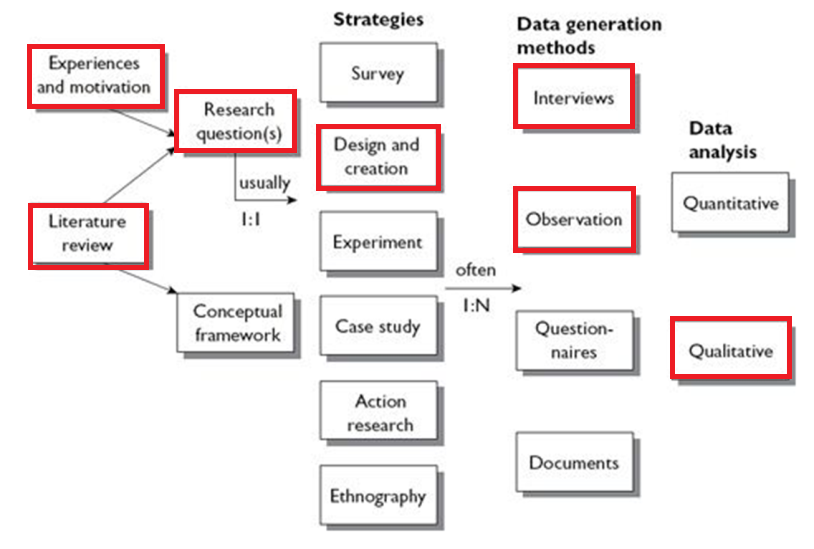
\includegraphics[width=0.42\textwidth]{fig/researchplan_image}
    \end{center}
    \caption{Model of the research process as illustrated in \citet{oates2006} }
    \label{researchplan_img}
\end{wrapfigure}

The research questions were derived through discussing the needs of the intended users with neuroscientists at the Kavli Institute. It was then narrowed down by a literature review, finding a lack of satisfactory substitutions for real brain dissections and especially finding no attempt at a practical multiplatform application for a more scalable use for students. The projects research question falls under the strategy of Design and Creation as the main goal is to develop a useful application for medical education. The focus on a smartphone solution was further motivated by the COVID-pandemic making from-home learning quite essential and making the passing around of HMD devices an unwanted scenario. As part of an agile software development model the gathering of qualitative data from observations and interviews within the scope of user testing will be essential. 

\subsection*{Development method}

\section{Contributions}
%% write about macro vs micro stuff

The research product resulting from this project will be a new computer-based software application using augmented reality and running on multiple platforms like HoloLens 1 and 2, Android and more. The aim will be to develop an application that can bridge the gap between expensive head mounted displays and everyday smartphones which you will find in the pocket of any student, and to use this as a collaborative tool for learning neuroanatomy. Throughout the development period we will consult with medical professionals and gather feedback from students on the usability of the application.

{
    \color{BrickRed}
    \noindent
    \newline
    Something about macro + micro
}

%%=========================================
\section{Limitations}

%%=========================================
\section{Outline}


% !TEX encoding = UTF-8 Unicode
%!TEX root = thesis.tex
% !TEX spellcheck = en-US
%%=========================================



\chapter{Background}

\section{Glossary?}

\section{Augmented Reality}
(Jentoft, 2020) AR can be defined as a system that fulfills three basic features: a combination of real and virtual worlds, real-time interaction, and accurate 3D registration of virtual and real objects.

\subsection*{AR, MR, XR, VR}\label{chap:armrxr}
As a new field, this field suffers from naming disagreements. This is a confusing reality which needs to be addressed. There are differing view of what each acronym refers to, and even what they stand for. I will overlook most of this discussion, and simply explain what is meant by each acronym in the scope of this project.

\paragraph*{AR}\label{para:ar} Augmented Reality, exercises which implement a see-through effect to display 3D visuals on top of the real-world. The idea of holograms is a good stand-in for the effect of AR. This is the term which will be most used in this project. 

\paragraph*{MR}\label{para:mr} Mixed Reality, anything within the spectrum between reality and pure visual 3D graphics, which blends computer generated visuals and reality. While the term was not invented by Microsoft\footnotemark, it is a term strongly associated with them, and in this project the term MR will generally only be used as a reference to Microsoft's products or concepts. There term is also used by some as a subset of \nameref{para:ar}, so in conclusion it is a somewhat controversial term. 

\footnotetext{In fact the term was coined by \citet{Milgram1994}, in this exact meaning.}
% That is at least what Microsoft is pushig for 

\paragraph*{XR}\label{para:xr} Extended Reality, much like \nameref{para:mr} this includes the whole spectrum of experiences blurring the line between the real and the virtual. However it does not have the Microsoft taint, nor the confusion of that term. And thus it is a more acceptable term, and it is what will be used here to describe the spectrum.

\paragraph*{VR}\label{para:vr} Virtual Reality, is enclosed experiences which completely surrounds the user within a computer generated world. This is a generally uncontroversial term and will be used for applications running on devices like the Oculus Rift and the HTC Vive.


\section{Graphics and Rendering}

\subsection*{Rasterization, Polygons and 3D models}

{
    \color{BrickRed}
    I feel that there is some misunderstanding about what a 3D model is.
    Maybe go in-depth about what I mean by 3D model. I have probably already used the term for different things.
}

\section{Neuro stuff}

\subsection*{Ethics of dissection}\label{chap:ethics}

\subsection*{The Waxholm Space Atlas of the Sprague Dawley Rat Brain}\label{chap:ratbrain}

{
    \color{BrickRed}
https://www.nitrc.org/projects/whs-sd-atlas
\begin{itemize}
    \item What is a atlas
    \item WHS and ratbrain is open, used and developed by NTNU St Olavs and UiO 
    \item Waxholm Space Atlas of the Sprague Dawley Rat Brain 
    \item Discuss difference between graphical 3D model and 3D atlas
\end{itemize}
}


%  In this pursuit we will also make use of high-resolution 3D imagery of a rat brain (see \autoref{chap:ratbrain}).  

This project makes use of high-resolution 3D-models of a rat brain. This brain model has been captured and manually delineated\footnotemark[1] by a collaboration between research groups at the University of Oslo and NTNU, and is in fact a highly accurate volumetric representations of the rat brain. This model is an open access community resource, intended as a free tool for education and research\footnotemark[2]. Within the convectional rasterization rendering pipe-line of Nevrolens, a polygonal asset derived from this volumetric model is naturally used. 

\footnotetext[1]{Delineation refers to the process of clearly defining different structures in the brain into separate namable parts.}
\footnotetext[2]{https://www.nitrc.org/projects/whs-sd-atlas}

The model is simply referred to as \textit{The Waxholm Space Atlas of the Sprague Dawley Rat Brain}. What follows is a brief explanation of each confusing part of the this name. 

\subsubsection*{Waxholm Space}\label{chap:whs}
\begin{wrapfigure}{R}{0.40\textwidth} 
    \centering
    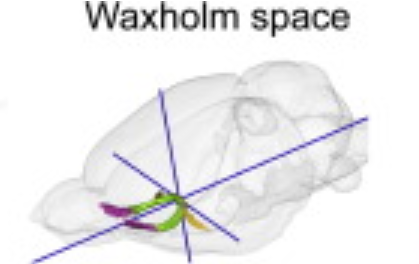
\includegraphics[width=0.30\textwidth]{fig/waxholmspace}
    \caption{\raggedright WHS \citep{WaxholmRatBrain2014}}
    \label{fig:waxholmspace}
\end{wrapfigure}

Waxholm Space (WHS) is a vector space defined as a standard reference space for the mouse brain and the rat brain \citep{WaxholmWithSimpleAbstract2013}. Its use as a coordinate system simplifies interoperability across atlases. It was developed by International Neuroinformatics Coordinating Facility (INCF) for the mouse brain, and has further been implemented in the rat brain by \citet{WaxholmRatBrain2014}. The following is the formal definition of WHS:


%  International Neuroinformatics Coordinating Facility (INCF) Digital Atlasing Project
\begin{quote}
\textit{
The coordinate system for WHS is defined as a continuous Cartesian system with the origin in the brain determined by 
\begin{itemize}
    \item the anterior commissure (AC) at the intersection between the mid sagittal plane,
    \item a coronal plane passing midway (rostro-caudal) through the anterior and posterior branches of AC, and
    \item a horizontal plane passing midway through the most dorsal and ventral aspect of the AC.
\end{itemize}
}
\citet{WaxholmSpaceAndMouseBrain2011}
\end{quote}

\noindent
\autoref{fig:waxholmspace} visualizes the axes through origin of WHS in the brain of a rat. Within the scope of this project WHS will be the local space of the rat brain model implemented in Nevrolens.

\subsubsection*{Brain Atlas}\label{chap:atlas}

A brain atlas is a composite representation based on one or more datasets of a given brain. An atlas generally has the function of highlighting some specified aspects and relations in the brain, and is a convectional tool in neuroscientific research \citep{Toga2000_AtlasBasics}. The convectional atlas is based on micrometer scale sliced sections in the brain, effectively creating two-dimensional layers through the brain. While functional, this "turns the brain into a book". Three-dimensional digital atlas are however relative newcomer on the neuro-imagery scene, by employing magnetic resonance imaging (MRI) and diffusion tensor imaging (DTI) the resulting atlases are complete volumetric representation of the subject brain \citep{WaxholmRatBrain2014}. 

This volumetric model is the basis for the delineated 3D-model used in Nevrolens.


\subsubsection*{Sprague Dawley}

Its a strain of laboratory rat.




\section{Equipment}

\subsection*{HoloLens 2}


\section{Tools}\label{chap:tools}


\subsection*{Unity}\label{chap:unity}
Unity is a game engine for developing 2D and 3D games. It has grown to become the most popular game engine used by single developers and small development teams because of its ease of use and simple licensing terms for independent developers. Because of its popularity  and ease of use Unity has become a platform for 3D development within more widespread fields than video gaming, such as engineering, moviemaking and architecture. 
Within this project the critical reason for choosing Unity for our 3D development is the exceptional support for the HoloLens product line. As seen in the \autoref{chap:mrtk}, Microsoft has poured resources into developing a "relatively" robust open framework for using Unity to develop for HoloLens. 
Alternatives to using Unity are slim, but one could be to use Unreal Engine, an 3D game engine with great support for VR and AR in general, however the support for HoloLens specific tools like \nameref{chap:mrtk} is limited\footnote{Microsoft has a version of MRTK for Unreal, called \href{https://github.com/microsoft/MixedRealityToolkit-Unreal}{MRTK-Unreal}. It seems to be stale however, not having any updates in the last six months in the time of writing.}.
% An alternative to using Unity wo

\subsection*{Mixed Reality Toolkit}\label{chap:mrtk}
Mixed Reality Toolkit (MRTK) is a open source, Microsoft-driven framework for Mixed Reality (MR) development. In practice it is Microsoft's SDK for HoloLens development, greatly simplifying development related to interaction, user interface and  [\dots]. As it is a framework for MR in general, it supports other platforms like Android, iOS and VR devices such as HTC Vive and Oculus Rift with OpenVR. 
An alternative to using MRTK would be to us XRTK which is a community-driven fork of MRKT. Thought such a choice would be an exercise of free software principles, it also lends it self to better support for some devices, like the MagicLeap.

\subsection*{Photon}\label{chap:photon}
Not in use jet

\subsection*{Blender}

\subsection*{Git}
Git flow, Gitmoji, GitKraken, Git gud 

\subsection*{GitKraken Boards}
Kanban and such \\
Used both / separately for Nevrolens and Project thesis.




\section{Related work}

\subsection*{VRVisualization}\label{chap:vrvis}

\subsection*{HoloAnatomy}

\subsection*{Insight Heart}

\subsection*{SphenoBlock?}

\subsection*{Noe HoloCare stuff?}


% !TEX encoding = UTF-8 Unicode
% !TEX root = ../thesis.tex
% !TEX spellcheck = en-US
%%=========================================



\chapter{Implementation}

% Hololens, UWP, WMR

\section{Requirements}

% cadavers difficult to get, vr -> less awareness
%
%


The first meeting initializing the project took place at VRLab Dragvoll in early September, here I was introduced to the general background and the problem description of how Witter and others envisioned the use of AR for neuroanatomical education. It was explained how cadavers for education are difficult to acquire and [\dots]. 
Another problem we discussed was related to the difference in medium between VR and AR. While the application \nameref{chap:vrvis} did have many of the features envisioned, and could have been a basis for further development. The fact that is was implemented in VR was problematic for the envisioned use cases. Being completely enclosed visually limits its use case in lectures and in any use case with collaboration in a physical space. Generally the loss of spatial awareness and eye contact as a result of using VR headsets was though of as an impediment for using VR for such an application. 
% something about the data set?
Thus, we had an outline of a neuroanatomical education tool in AR using the HoloLens 2 and concluded with some questions and requirements for the project:

\begin{enumerate}\label{mennoslist}
    \item Can the current VR dataset\footnotemark be used in the HoloLens 2 AR environment?
    \item If not, which steps need to be taken to use the segmented WHS rat brain to develop a suitable 3D model that can be used in AR?
    \item Develop an optimal user interface for a single person to explore the rat brain as if the user is doing a dissection of a real brain.
    \item Develop/test ways to make this a multiuser/shareable tool adequate in a teaching environment.
    \item Explore ways to integrate microscopical data into the AR representation.
    \item Describe/explore the feasibility to implement the system for Human neuroanatomy education.
\end{enumerate}

\footnotetext{Referring to \nameref{chap:vrvis}.}

Here items 1-4 were deemed critical for the project, while 5 and 6 were dependent on the progress made.

This meeting together with the list formed a clear problem description and can be seen as the initial discovery process of the project. Though the following period of exploring the newly arrived HoloLens 2 and its capabilities, we formed a set of \textit{system requirements}. 
System requirements are descriptions of how a system should operate, what it should be able to do and the constraints of its operation. The requirements must reflect the stakeholders needs for the system \citep{PUboka}. System requirements are generally split into functional requirements, which describe specifics of what the system (and its sub-systems) should do, and non-functional requirements, which generally are descriptions of the user experience of the system as a whole. 
What follows are the system requirements decided on for the application: 

\subsection*{Functional Requirements}
\begin{enumerate}
    \item {
        \textbf{Implement a brain dissection tool in AR}\\
         
    }
    \item {
        \textbf{The application must run in HoloLens 2 and a mobile platform}\\
         Android and/or iOS
    }

    \item {
        \textbf{Collaboration}\\
         
    }

\end{enumerate}

\subsection*{Non-Functional Requirements}

\begin{enumerate}
    \item 
\end{enumerate}

% and non-functional requirements, which describe  










\section{Software Process}
% https://www.wikipendium.no/TDT4140_Programvareutvikling/nb/#kapittel-2-software-processes

% Incremental development etc. \#agile
\large{Where everything I learned in PU should shine!}

Even though I have developed the Nevrolens application by myself, I have strived to use best practices for a software development workflow. These practices have generally grown out of the the needs of a multi-developer setting, to simplify the needs for collaboration and version control. Though their value possibly increases exponentially by the number of team members, I have found value in the structure and clarity I find in the workflow. 
My workflow consist of 




\section{Validation / Testing}



% !TEX encoding = UTF-8 Unicode
%!TEX root = thesis.tex
% !TEX spellcheck = en-US
%%=========================================



\chapter{Results}\label{chap:results}




The results in this research project are mainly gathered from the final test session, which was held after the last development stage, thus the results reflect the state of the application at the end of the research. 

The test sessions had two separate qualitative data gathering strategies: 

A multiple choice knowledge test taken by the test participants before and after the session,  this was meant to demonstrate learning value in short term time frame. Such a simple short term test could support the claim that the artifact can be used as an educational tool. The test is attached as \autoref{chap:knowtest}.
The second strategy was a combined SUS questionnaire with general questions about the application. This questionnaire can be found as \autoref{chap:questionnaire}.
The knowledge test was taken by the medical students in test sessions, while the questionnaire was answered by six participants, of which four were medical students.

% though further research is needed.

\section{Neuroanatomical test}
The multiple choice neuroanatomical knowledge test was performed at both test sessions. The test was taken by three medical students at the first session, two third year and one fifth year student. At the second session five first year medical students partook in the knowledge test.

\begin{figure}[H]
    \centering
    \begin{subfigure}[t]{0.8\textwidth}
        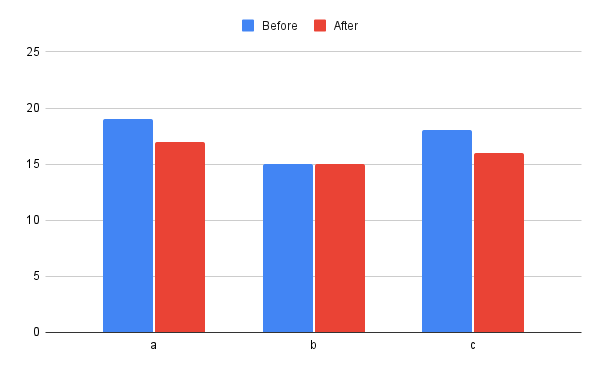
\includegraphics[width=\textwidth]{fig/knowtestresult1}
        \caption{}
    \end{subfigure}
    \begin{subfigure}[b]{0.8\textwidth}
        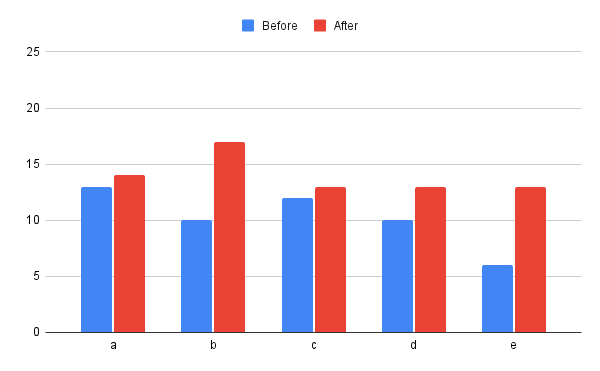
\includegraphics[width=\textwidth]{fig/knowtestresult2}
        \caption{}
    \end{subfigure}
\end{figure}





\section{Questionnaire}

The usability results are based on the second test session where a questionnaire, including a SUS section, was uses in addition to unstructured feedback from the test participants. The results from these methods will be presented in this section. 

\subsection{System usability scale questionnaire}
 
The SUS questionnaire was taken by six participants, five answering based on the HoloLens 2 experience and one based on using the Android application. The mean score from the HoloLens 2 is $79.0 \pm 10.4$, while the result from the single Android test was 75. This means that the application on HoloLens 2 sits high in the good rating almost reaching excellent, while the Android app is near the middle of the good rating. \autoref{fig:susresults} show the results of the SUS questionnaire charted with the red line representing the 68 \textit{average} score. All answers are listed in \autoref{tab:sus}, note that SUS is ordered such that every other statement is negative, meaning that a better score is achieved when they are disagreed to.

% Please add the following required packages to your document preamble:
% \usepackage[table,xcdraw]{xcolor}
% If you use beamer only pass "xcolor=table" option, i.e. \documentclass[xcolor=table]{beamer}
\begin{table}[]
    
\centering
\textbf{Results from SUS questionnaire}\par\medskip
\small
\begin{tabular}{l|ccccc}
\hline
                                                                                                                                         & \begin{tabular}[c]{@{}c@{}}Strongly\\ disagree\end{tabular} & Disagree                                                   & Neutral                                                    & Agree                                                     & \begin{tabular}[c]{@{}c@{}}Strongly\\ agree\end{tabular}   \\ \hline
\begin{tabular}[c]{@{}l@{}}I think that I would like to use this \\ system frequently.\end{tabular}                                      & {\color[HTML]{333333} \textbf{}}                            & {\color[HTML]{333333} \textbf{}}                           & {\color[HTML]{333333} \textbf{}}                           & \cellcolor[HTML]{9698ED}{\color[HTML]{EFEFEF} \textbf{2}} & \cellcolor[HTML]{6434FC}{\color[HTML]{EFEFEF} \textbf{4*}} \\
\rowcolor[HTML]{EFEFEF} 
\begin{tabular}[c]{@{}l@{}}I found the system \\ unnecessarily complex.\end{tabular}                                                     & \cellcolor[HTML]{6665CD}{\color[HTML]{EFEFEF} \textbf{3}}   & \cellcolor[HTML]{9698ED}{\color[HTML]{EFEFEF} \textbf{2*}} & \cellcolor[HTML]{CBCEFB}{\color[HTML]{EFEFEF} \textbf{1}}  & {\color[HTML]{333333} \textbf{}}                          & {\color[HTML]{333333} \textbf{}}                           \\
\begin{tabular}[c]{@{}l@{}}I thought the system was \\ easy to use.\end{tabular}                                                         & {\color[HTML]{333333} \textbf{}}                            & {\color[HTML]{333333} \textbf{}}                           & \cellcolor[HTML]{9698ED}{\color[HTML]{EFEFEF} \textbf{2*}} & \cellcolor[HTML]{6434FC}{\color[HTML]{EFEFEF} \textbf{4}} & {\color[HTML]{333333} \textbf{}}                           \\
\rowcolor[HTML]{EFEFEF} 
\begin{tabular}[c]{@{}l@{}}I think that I would need the \\ support of a technical person \\ to be able to use this system.\end{tabular} & \cellcolor[HTML]{6665CD}{\color[HTML]{EFEFEF} \textbf{3*}}  & \cellcolor[HTML]{9698ED}{\color[HTML]{EFEFEF} \textbf{2}}  & \cellcolor[HTML]{CBCEFB}{\color[HTML]{EFEFEF} \textbf{1}}  & {\color[HTML]{333333} \textbf{}}                          & {\color[HTML]{333333} \textbf{}}                           \\
\begin{tabular}[c]{@{}l@{}}I found the various functions in \\ this system were well integrated.\end{tabular}                            & {\color[HTML]{333333} \textbf{}}                            & {\color[HTML]{333333} \textbf{}}                           & \cellcolor[HTML]{CBCEFB}{\color[HTML]{EFEFEF} \textbf{1*}} & \cellcolor[HTML]{6434FC}{\color[HTML]{EFEFEF} \textbf{4}} & \cellcolor[HTML]{CBCEFB}{\color[HTML]{EFEFEF} \textbf{1}}  \\
\cellcolor[HTML]{EFEFEF}\begin{tabular}[c]{@{}l@{}}I thought there was too much \\ inconsistency in this system.\end{tabular}            & \cellcolor[HTML]{CBCEFB}{\color[HTML]{EFEFEF} \textbf{1}}   & \cellcolor[HTML]{6665CD}{\color[HTML]{EFEFEF} \textbf{3}}  & \cellcolor[HTML]{CBCEFB}{\color[HTML]{EFEFEF} \textbf{1}}  & \cellcolor[HTML]{CBCEFB}{\color[HTML]{EFEFEF} \textbf{1*}}   & \cellcolor[HTML]{EFEFEF}\textbf{}                          \\
\begin{tabular}[c]{@{}l@{}}I would imagine that most \\ people would learn to use \\ this system very quickly.\end{tabular}              & {\color[HTML]{333333} \textbf{}}                            & {\color[HTML]{333333} \textbf{}}                           & \cellcolor[HTML]{CBCEFB}{\color[HTML]{EFEFEF} \textbf{1}}  & \cellcolor[HTML]{6665CD}{\color[HTML]{EFEFEF} \textbf{3}} & \cellcolor[HTML]{9698ED}{\color[HTML]{EFEFEF} \textbf{2*}} \\
\rowcolor[HTML]{EFEFEF} 
\begin{tabular}[c]{@{}l@{}}I found the system very \\ cumbersome to use.\end{tabular}                                                    & \cellcolor[HTML]{9698ED}{\color[HTML]{EFEFEF} \textbf{2}}   & \cellcolor[HTML]{6665CD}{\color[HTML]{EFEFEF} \textbf{3}}  & \cellcolor[HTML]{CBCEFB}{\color[HTML]{EFEFEF} \textbf{1*}} & {\color[HTML]{333333} \textbf{}}                          & {\color[HTML]{333333} \textbf{}}                           \\
\begin{tabular}[c]{@{}l@{}}I felt very confident using \\ the system.\end{tabular}                                                       & {\color[HTML]{333333} \textbf{}}                            & {\color[HTML]{333333} \textbf{}}                           & \cellcolor[HTML]{CBCEFB}{\color[HTML]{EFEFEF} \textbf{1}}  & \cellcolor[HTML]{9698ED}{\color[HTML]{EFEFEF} \textbf{2}} & \cellcolor[HTML]{6665CD}{\color[HTML]{EFEFEF} \textbf{3*}} \\
\rowcolor[HTML]{EFEFEF} 
\begin{tabular}[c]{@{}l@{}}I needed to learn a lot of \\ things before I could get \\ going with this system.\end{tabular}               & \cellcolor[HTML]{9698ED}{\color[HTML]{EFEFEF} \textbf{2*}}  & \cellcolor[HTML]{6665CD}{\color[HTML]{EFEFEF} \textbf{3}}  & {\color[HTML]{333333} \textbf{}}                           & \cellcolor[HTML]{CBCEFB}{\color[HTML]{EFEFEF} \textbf{1}} & {\color[HTML]{333333} \textbf{}}                           \\ \hline
\end{tabular}
\caption{The results form the SUS section. Number and color values represent the magnitude of answers with the corresponding alternative. Android answer is marked with "*".}
\label{tab:sus}

\end{table}

\begin{figure}
    \centering
    \textbf{SUS results}\par\medskip
    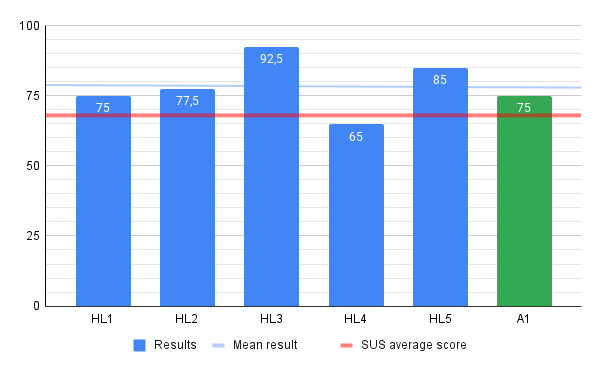
\includegraphics[width=0.75\textwidth]{fig/susbarchart}
    \caption{The blue results are from HoloLens 2, while the green is from Android.}
    \label{fig:susresults}
\end{figure}


\subsection{Research specific questionnaire}\label{chap:researchspes}
The questionnaire included a section with research specific questions written by the researcher with the aim to gather data relating to the research questions of the project. The question were, just as in SUS, based on the \textit{Likert scale}, with answer alternatives ranging from 1 - 5 indicating how much in agreement the user is with the statement. The section was answered by six participants, and it was platform independent. The results can be seen in \autoref{tab:researchspes}. In addition to the Likert ranking free form text boxes were provided after the questions for gathering qualitative data. 


% Notably, the participants were asked what platform they preferred
Notably, every participant who tried both platforms preferred the HoloLens 2 experience, based on the question \textit{Which platform did you prefer?}. Saying the following:
\newline
\textbf{Why did you prefer that platform?}
{\small\itshape
\begin{itemize}[]
    \item Physically interactive and the menu is on your hand
    \item Much easier to understand the 3d structure, as you can see and rotate it at any angle.
    \item Holo is easier to manoeuvre and look from different angles.
    \item It was more a more fun way of learning, which again increases motivation for learning.
\end{itemize}
}

% Please add the following required packages to your document preamble:
% \usepackage[table,xcdraw]{xcolor}
% If you use beamer only pass "xcolor=table" option, i.e. \documentclass[xcolor=table]{beamer}
% \usepackage[normalem]{ulem}
% \useunder{\uline}{\ul}{}
\begin{table}[h]
\centering
\textbf{Results from research questionnaire}\par\medskip
\small
\begin{tabular}{l|ccccc}
\hline
                                                                                                                                                          & \begin{tabular}[c]{@{}c@{}}Strongly\\ disagree\end{tabular} & Disagree                                                  & Neutral                                                   & Agree                                                     & \begin{tabular}[c]{@{}c@{}}Strongly\\ agree\end{tabular}  \\ \hline
\begin{tabular}[c]{@{}l@{}}I got new insight about neuroanatomy \\ while using the system.\end{tabular}                                                   & \textbf{}                                                   & \textbf{}                                                 & \textbf{}                                                 & \cellcolor[HTML]{6434FC}{\color[HTML]{EFEFEF} \textbf{4}} & \cellcolor[HTML]{9698ED}{\color[HTML]{EFEFEF} \textbf{2}} \\
\rowcolor[HTML]{EFEFEF} 
\begin{tabular}[c]{@{}l@{}}I got new insight about neuroanatomy \\ while seeing and manipulating the \\ brain and its structures in 3D.\end{tabular}      & \textbf{}                                                   & \textbf{}                                                 & \textbf{}                                                 & \cellcolor[HTML]{9698ED}{\color[HTML]{EFEFEF} \textbf{2}} & \cellcolor[HTML]{6434FC}{\color[HTML]{EFEFEF} \textbf{4}} \\
\begin{tabular}[c]{@{}l@{}}I got new insight about neuroanatomy \\ while dissecting the brain.\end{tabular}                                               & \textbf{}                                                   & \textbf{}                                                 & \cellcolor[HTML]{CBCEFB}{\color[HTML]{EFEFEF} \textbf{1}} & \cellcolor[HTML]{6200C9}{\color[HTML]{EFEFEF} \textbf{5}} & \textbf{}                                                 \\
\rowcolor[HTML]{EFEFEF} 
\cellcolor[HTML]{EFEFEF}\begin{tabular}[c]{@{}l@{}}I felt like I was collaborating with another \\ person when using the system with others.\end{tabular} & \cellcolor[HTML]{CBCEFB}{\color[HTML]{EFEFEF} \textbf{1}}                           & \cellcolor[HTML]{CBCEFB}{\color[HTML]{EFEFEF} \textbf{1}}                         & \cellcolor[HTML]{6665CD}{\color[HTML]{EFEFEF} \textbf{3}} & \cellcolor[HTML]{CBCEFB}{\color[HTML]{EFEFEF} \textbf{1}}                         & \cellcolor[HTML]{EFEFEF}\textbf{}                         \\
\begin{tabular}[c]{@{}l@{}}I was aware of what the other person did \\ and had focus on when using the system.\end{tabular}                               & \textbf{}                                                   & \cellcolor[HTML]{9698ED}{\color[HTML]{EFEFEF} \textbf{2}} & \cellcolor[HTML]{6665CD}{\color[HTML]{EFEFEF} \textbf{3}} & \cellcolor[HTML]{CBCEFB}{\color[HTML]{EFEFEF} \textbf{1}} & \textbf{}                                                 \\
\rowcolor[HTML]{EFEFEF} 
\begin{tabular}[c]{@{}l@{}}The system would be useful for remote \\ teaching of neuroanatomy.\end{tabular}                                                & \textbf{}                                                   & \textbf{}                                                 & \cellcolor[HTML]{CBCEFB}{\color[HTML]{EFEFEF} \textbf{1}} & \cellcolor[HTML]{9698ED}{\color[HTML]{EFEFEF} \textbf{2}} & \cellcolor[HTML]{6665CD}{\color[HTML]{EFEFEF} \textbf{3}} \\ \hline
\end{tabular}
\caption{The results form the research specific questions, the number and color values represent the magnitude of answers with the corresponding alternative.}
\label{tab:researchspes}
\end{table}

\subsection{IPEAR AR and peer learning questionnaire}
This section was included as part of other research at the NTNU VRLab. The results from the section is however just as relevant for this study. \autoref{tab:peer} shows the results.

\begin{table}[]
\centering
\textbf{Results from AR and peer learning questionnaire}\par\medskip
\small
\begin{tabular}{l|ccccc}
\hline
                                                                                                                                             & \begin{tabular}[c]{@{}c@{}}Strongly\\ disagree\end{tabular} & Disagree                                                  & Neutral                                                   & Agree                                                     & \begin{tabular}[c]{@{}c@{}}Strongly\\ agree\end{tabular}  \\ \hline
\begin{tabular}[c]{@{}l@{}}Did you like the approach of peer learning \\ \small{(working with and teaching your classmates)}?\end{tabular}           & \textbf{}                                                   & \textbf{}                                                 & \cellcolor[HTML]{6665CD}{\color[HTML]{EFEFEF} \textbf{3}} &  & \cellcolor[HTML]{6665CD}{\color[HTML]{EFEFEF} \textbf{3}} \\
\rowcolor[HTML]{EFEFEF} 
\begin{tabular}[c]{@{}l@{}}Were you more interested in teaching \\each other  and sharing content with \\your peers and AR tools?\end{tabular} & \textbf{}                                                   & \cellcolor[HTML]{CBCEFB}{\color[HTML]{EFEFEF} \textbf{1}} & \cellcolor[HTML]{CBCEFB}{\color[HTML]{EFEFEF} \textbf{1}} & \cellcolor[HTML]{6434FC}{\color[HTML]{EFEFEF} \textbf{4}} & {\color[HTML]{EFEFEF} \textbf{}}                          \\
\begin{tabular}[c]{@{}l@{}}Did this learning approach make you feel \\ more responsible for your learning?\end{tabular}                      & \textbf{}                                                   & \cellcolor[HTML]{CBCEFB}{\color[HTML]{EFEFEF} \textbf{1}} & \cellcolor[HTML]{6665CD}{\color[HTML]{EFEFEF} \textbf{3}} & \cellcolor[HTML]{CBCEFB}{\color[HTML]{EFEFEF} \textbf{1}} & \cellcolor[HTML]{CBCEFB}{\color[HTML]{EFEFEF} \textbf{1}} \\
\rowcolor[HTML]{EFEFEF} 
\begin{tabular}[c]{@{}l@{}}Do you think it would be useful in other \\ courses or fields of study as well?\end{tabular}                      & {\color[HTML]{EFEFEF} \textbf{}}                            & {\color[HTML]{EFEFEF} \textbf{}}                          & {\color[HTML]{EFEFEF} \textbf{}}                          & \cellcolor[HTML]{9698ED}{\color[HTML]{EFEFEF} \textbf{2}} & \cellcolor[HTML]{6434FC}{\color[HTML]{EFEFEF} \textbf{4}} \\ \hline
\end{tabular}
\caption{The results form the research specific questions, the number and color values represent the magnitude of answers with the corresponding alternative.}
\label{tab:peer}
\end{table}


\subsection{Feedback from participants}

During the test sessions the participants gave feedback on their thoughts of the application, and how to improve the user experience. For the HoloLens 2 application the stated feedback was overwhelmingly positive, in \autoref{chap:researchspes} some give more constructive feedback which was not pointed out when talking with the participants. For the Android experience the prime vocalized feedback was to disable the AR in the application such that it would be a standard 3D application, this was explained both by the poor spatial locking on the device and the non optimal ergonomics of having to point the camera on the same spot at all times. 





%====================================================

% % The result of this project is the preliminary work for my master thesis next semester, thus 

% \section{Nevrolens}\label{nevrolens}
% Nevrolens is the name I've given the application which is the research product of this project. It's a combination of the Norwegian word Nevroanatomi and HoloLens. It is a AR application running on HoloLens 1, HoloLens 2 and Android. 

% The application is focused on delivering a single user experience, with features as cutting planes, scaling, moving brain parts and transparent brain parts. \autoref{fig:nevrolens_holo} show these features running on HoloLens 2, while \autoref{fig:nevrolens_android} show them on Android.
% It is packages and released on GitLab at \url{https://gitlab.stud.idi.ntnu.no/imtel/nevrolens}. 

% \begin{figure}[h]\label{fig:nevrolens_holo}
%     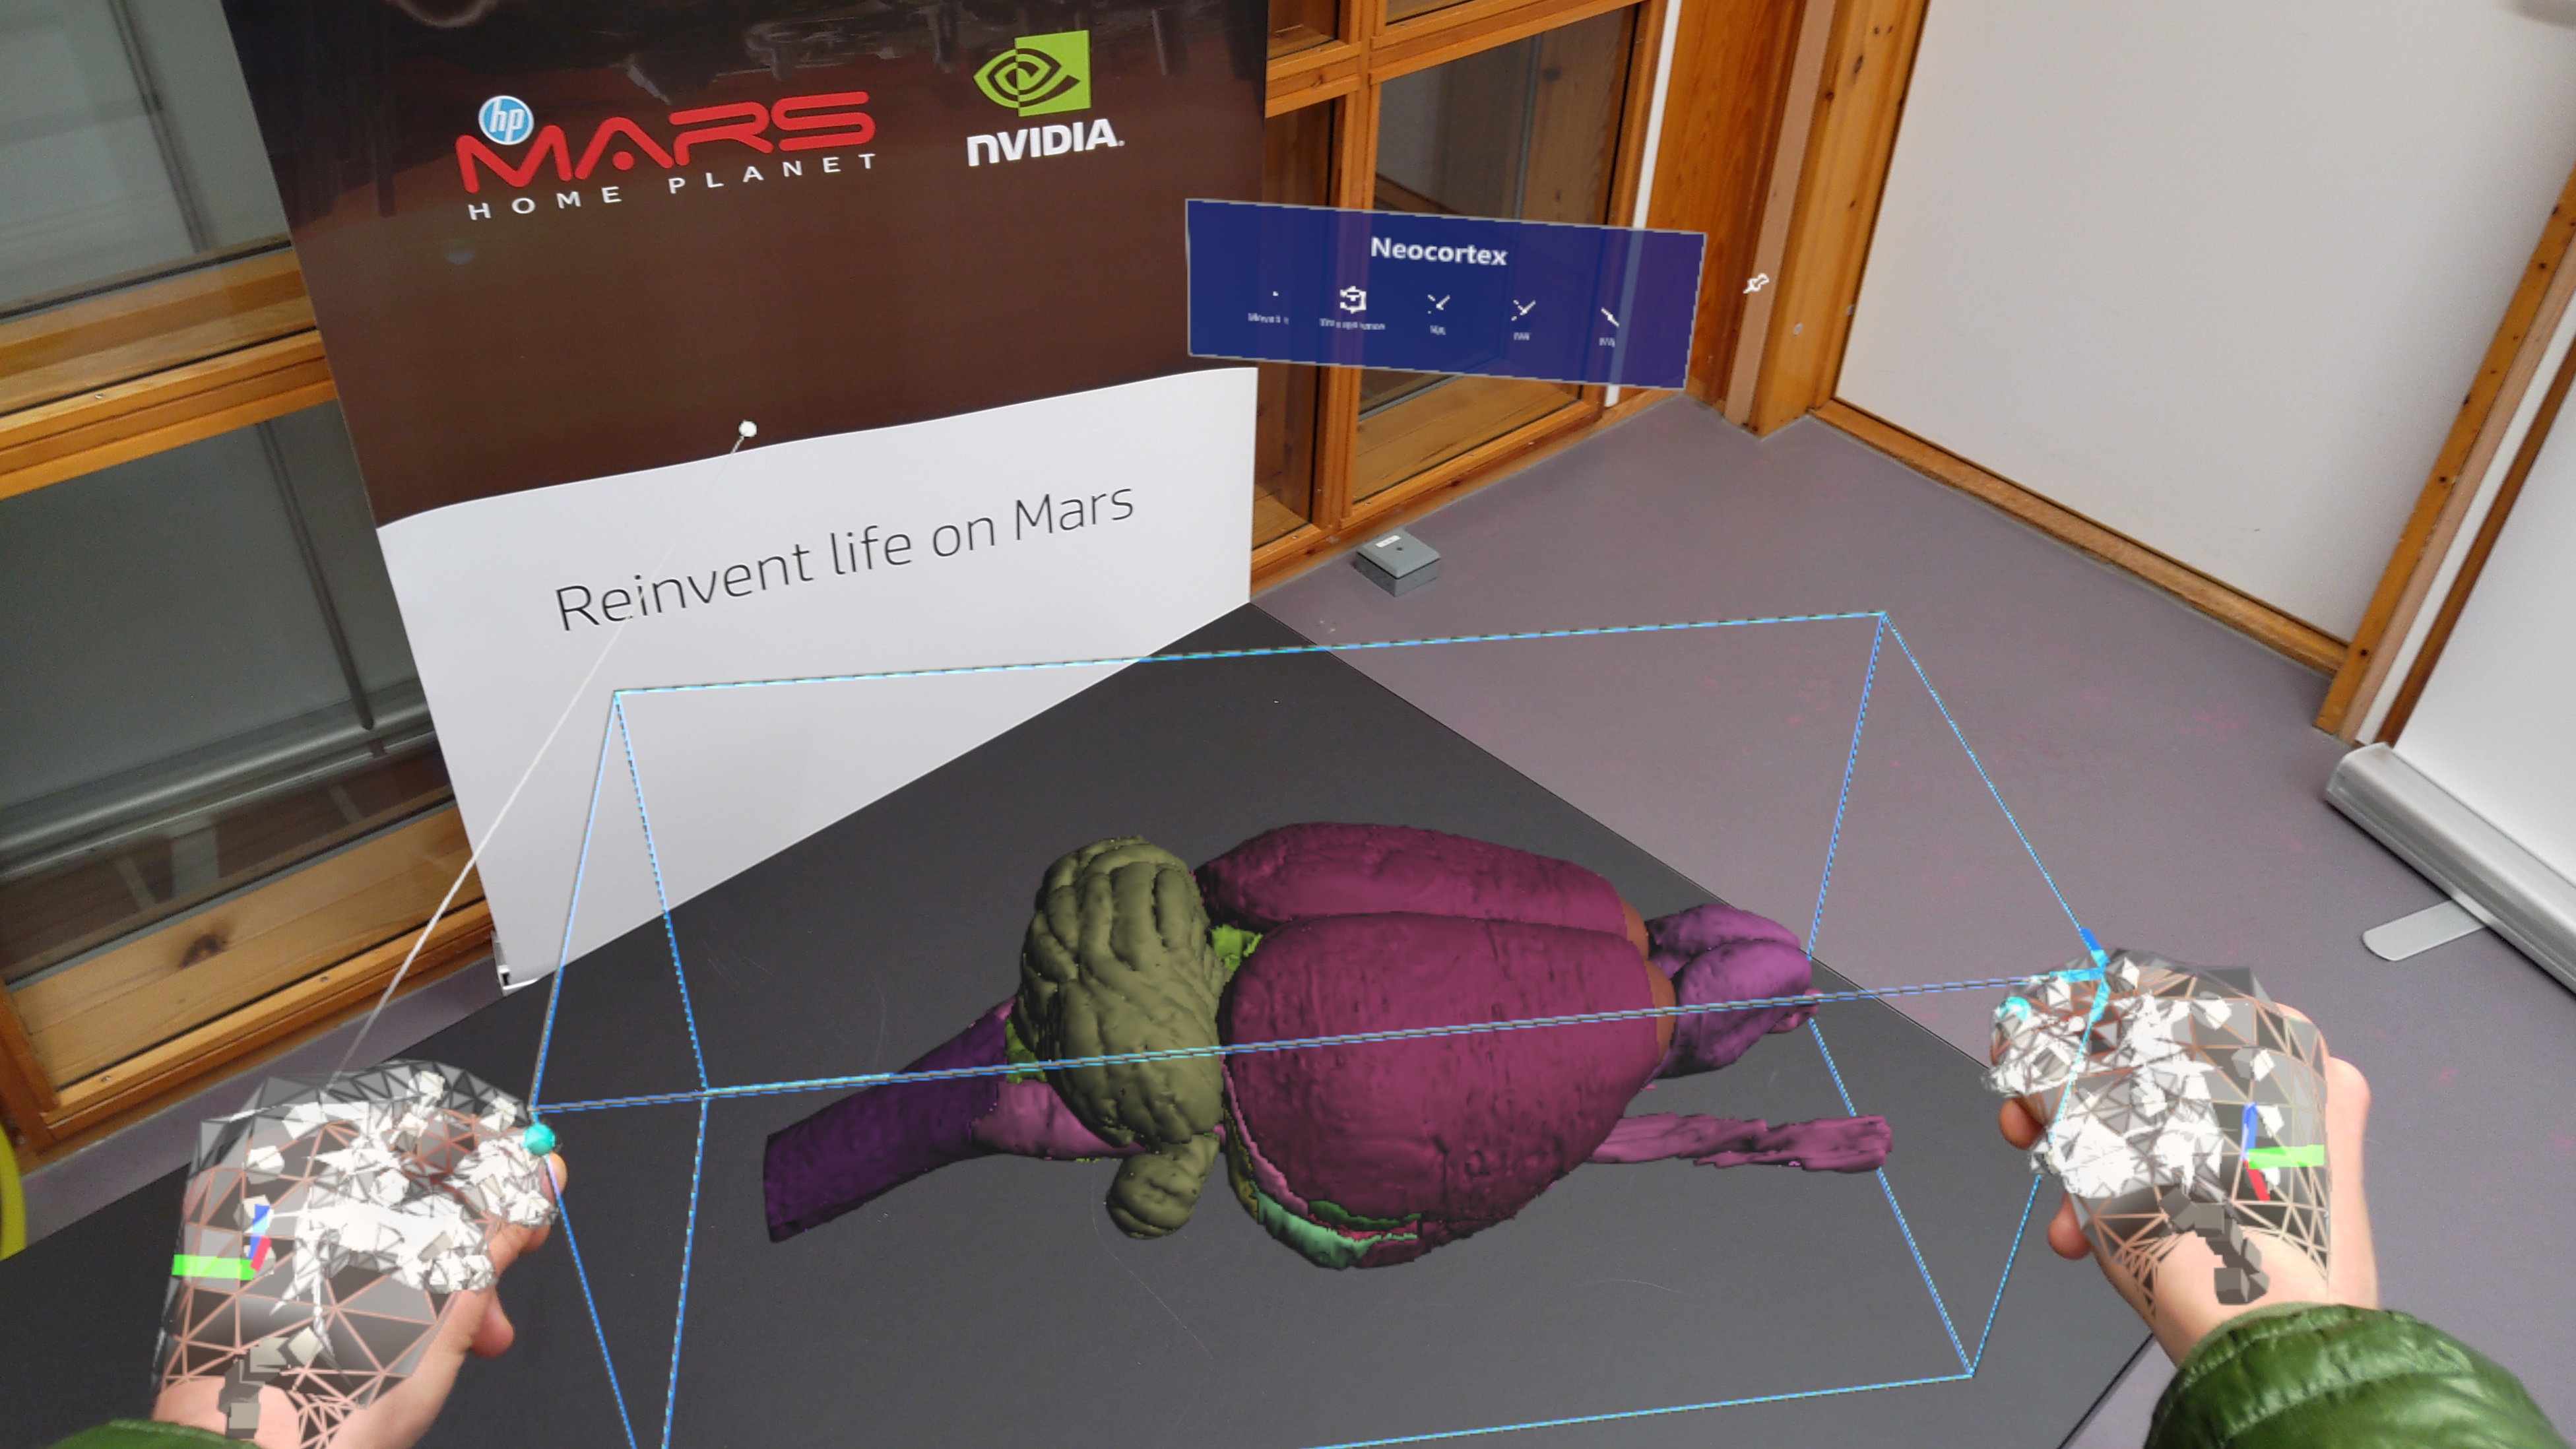
\includegraphics[width=0.5\textwidth]{fig/nevrolens/twohandedzoom.jpg}
%     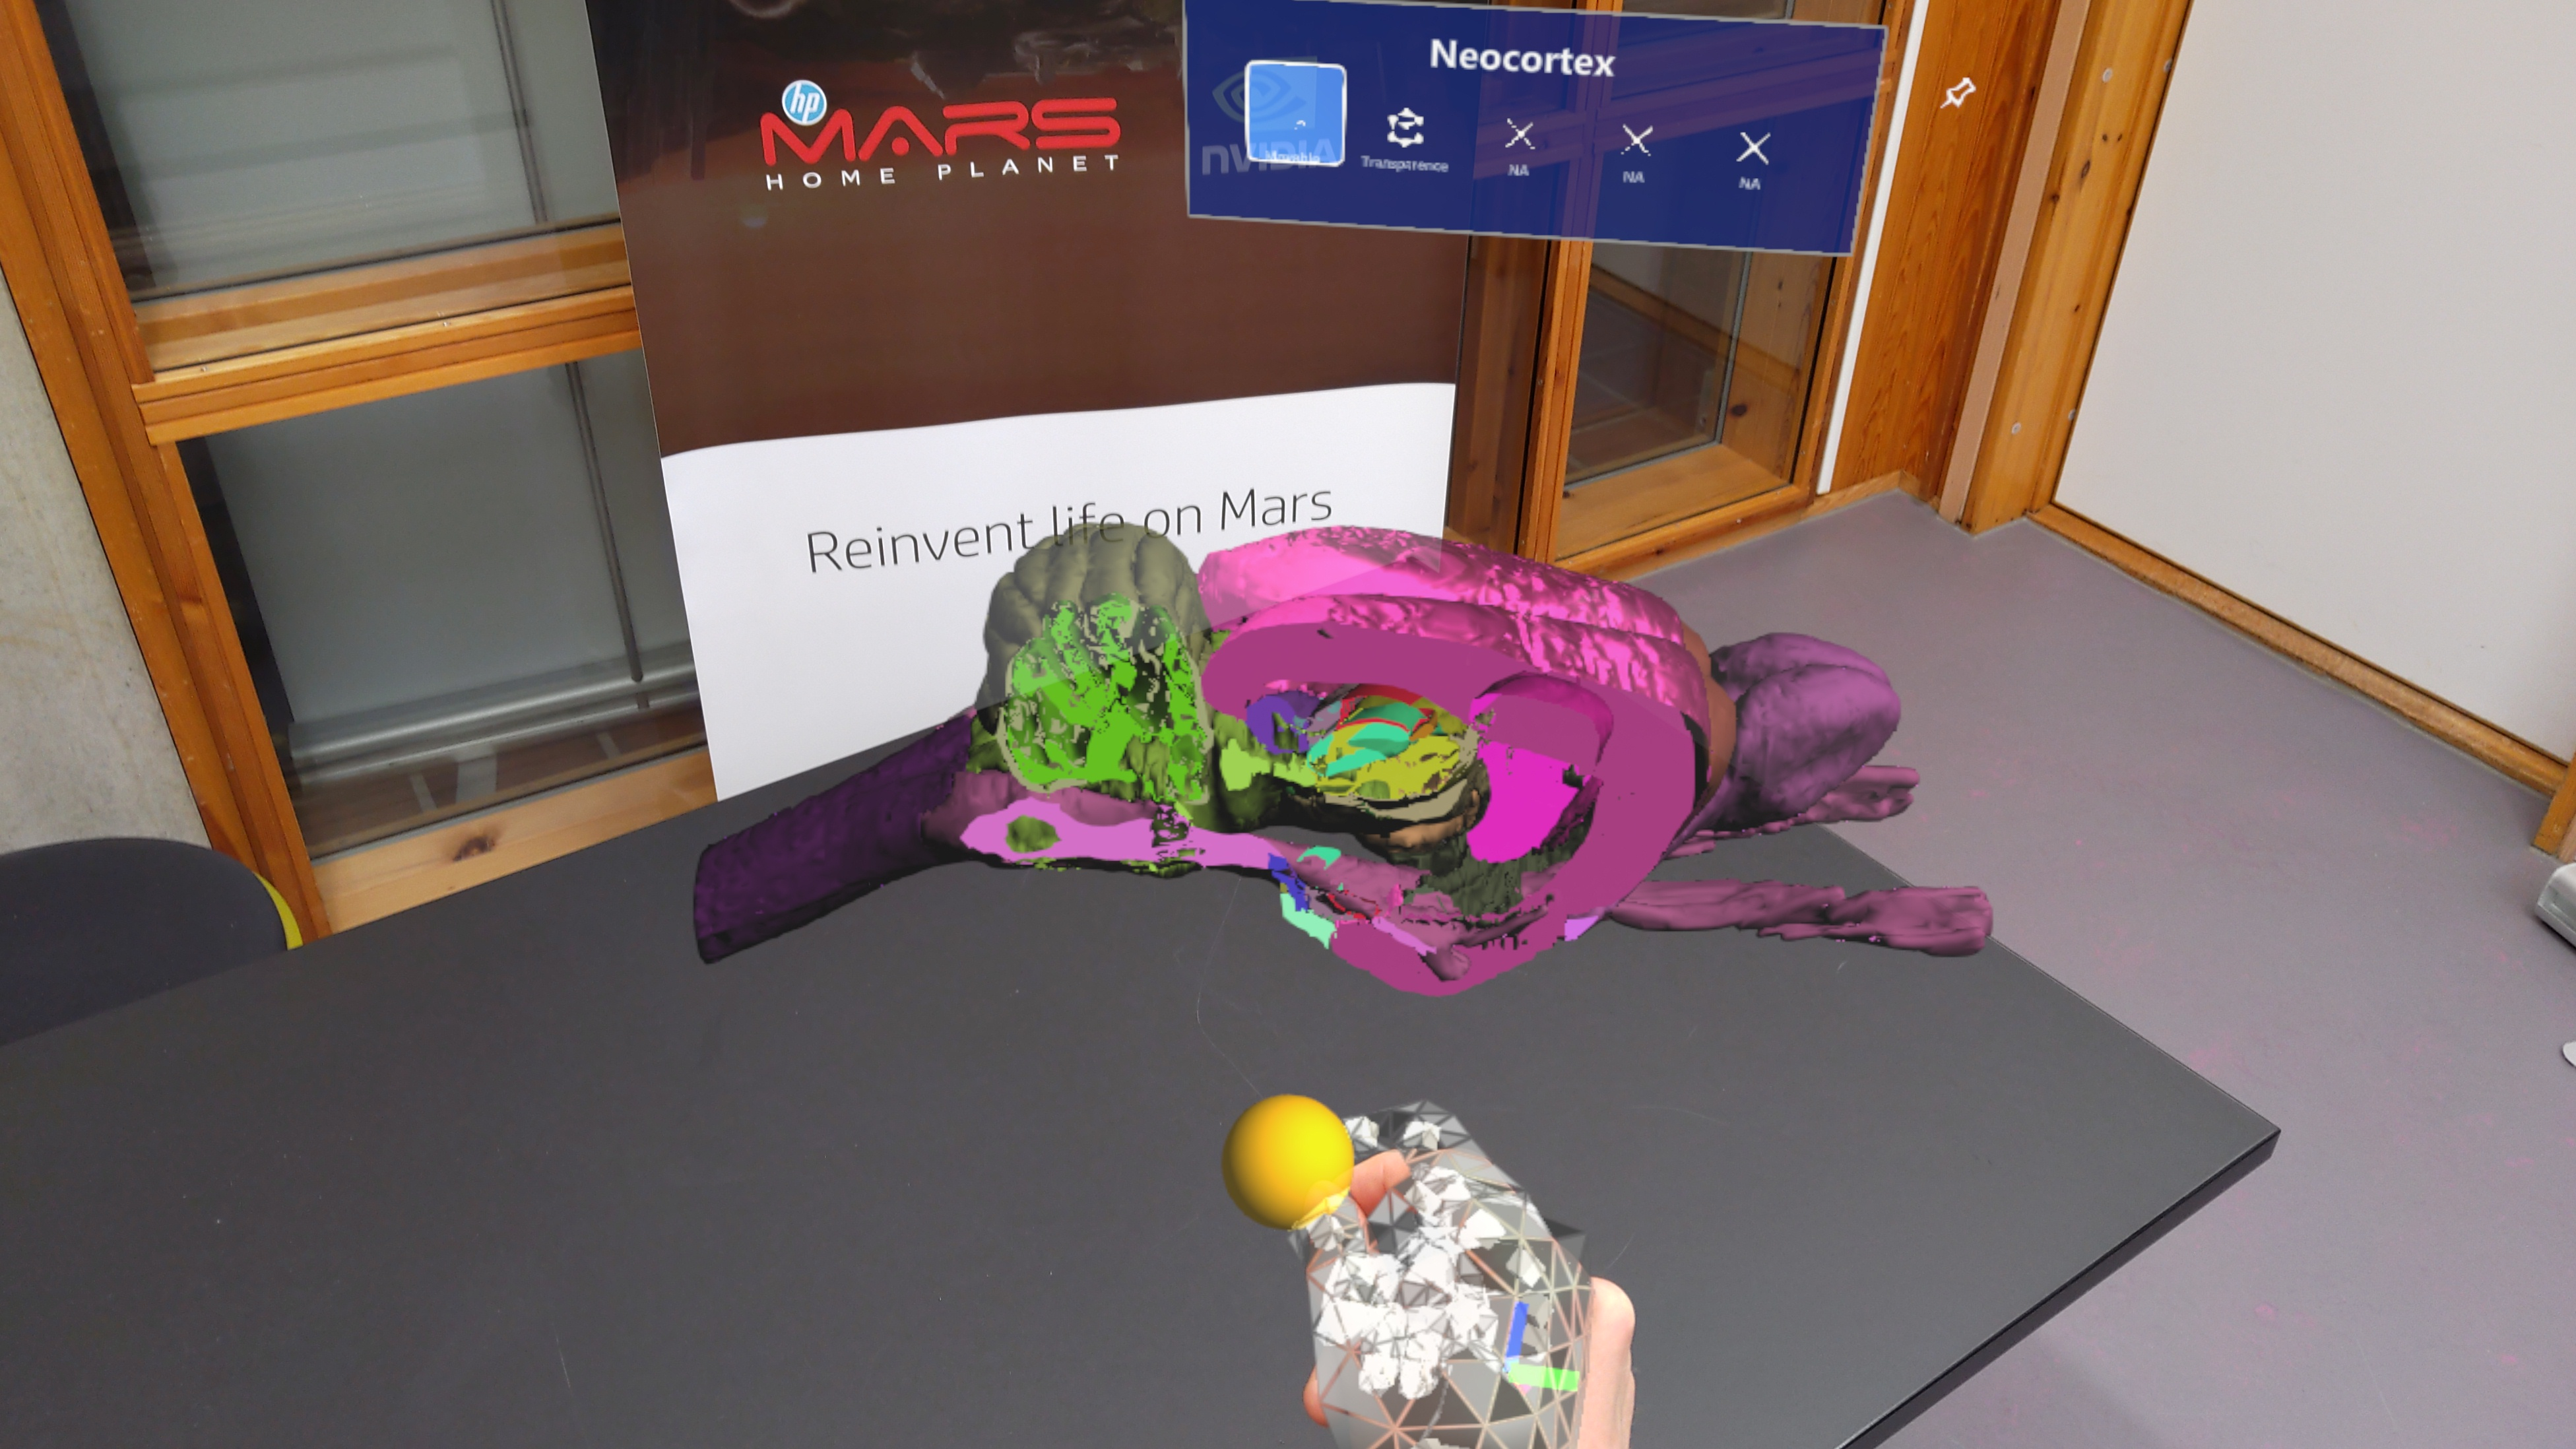
\includegraphics[width=0.5\textwidth]{fig/nevrolens/clipping.jpg}
%     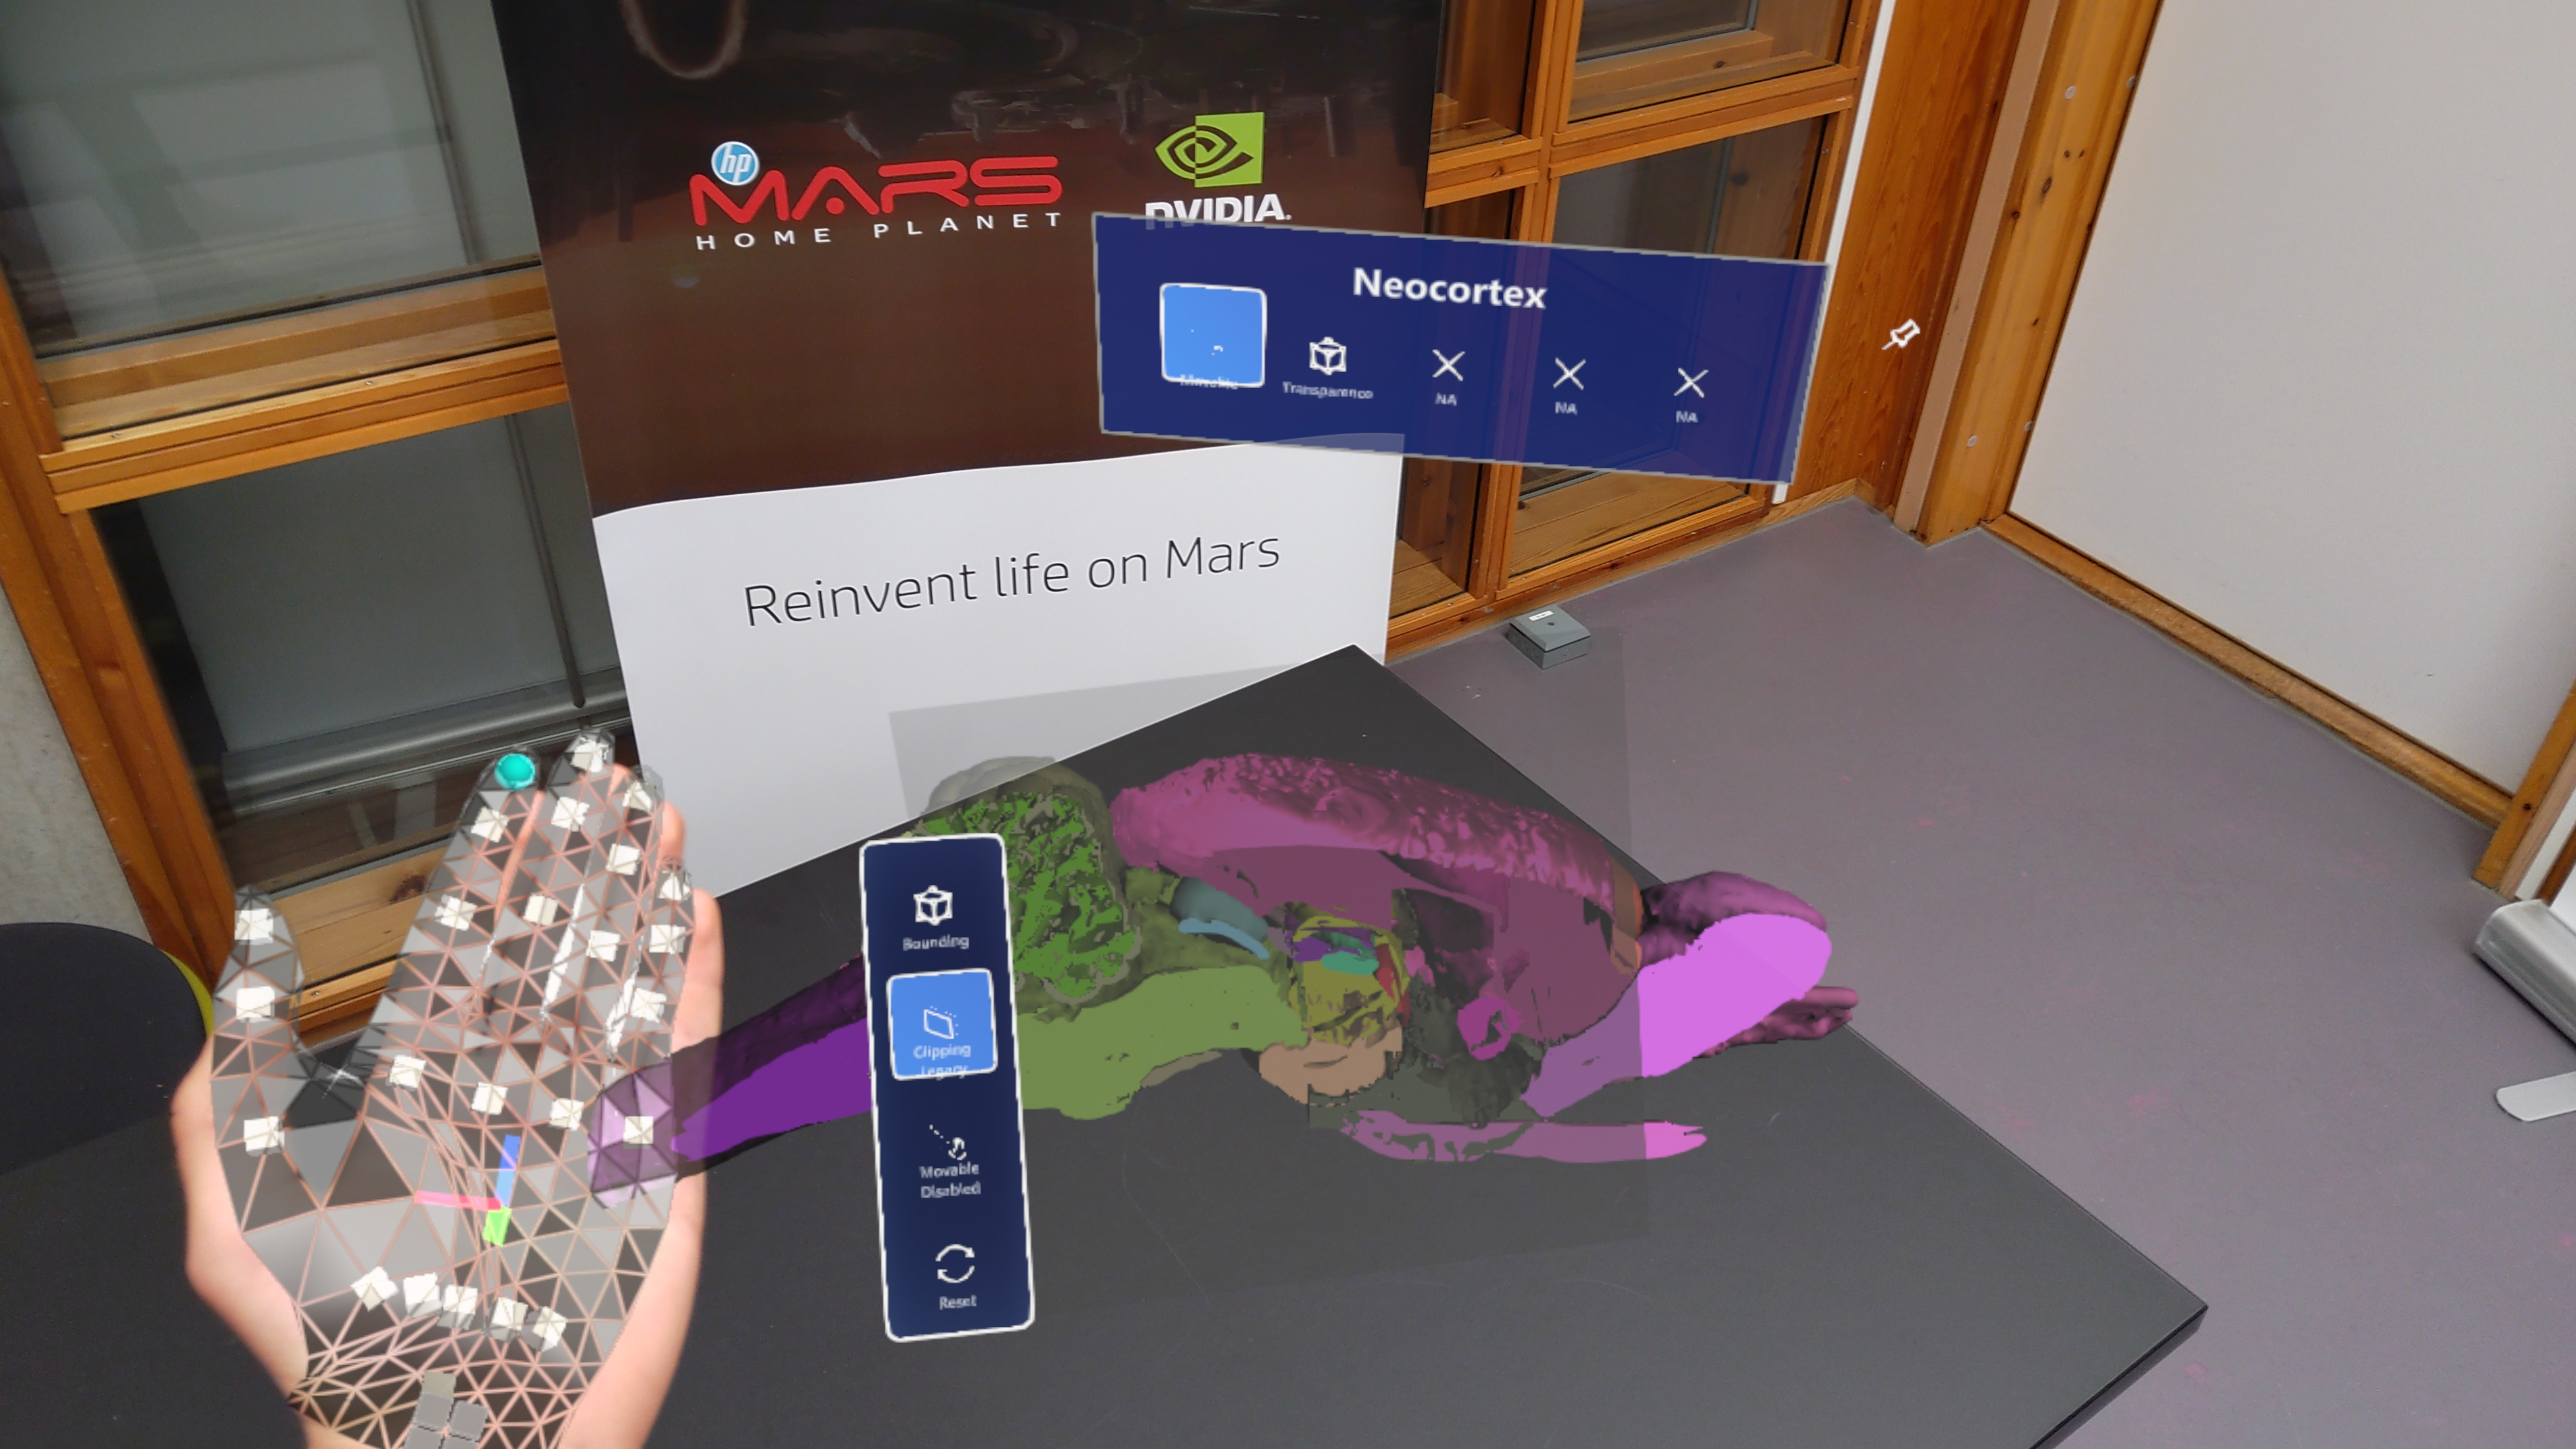
\includegraphics[width=0.5\textwidth]{fig/nevrolens/palmmenu.jpg}
%     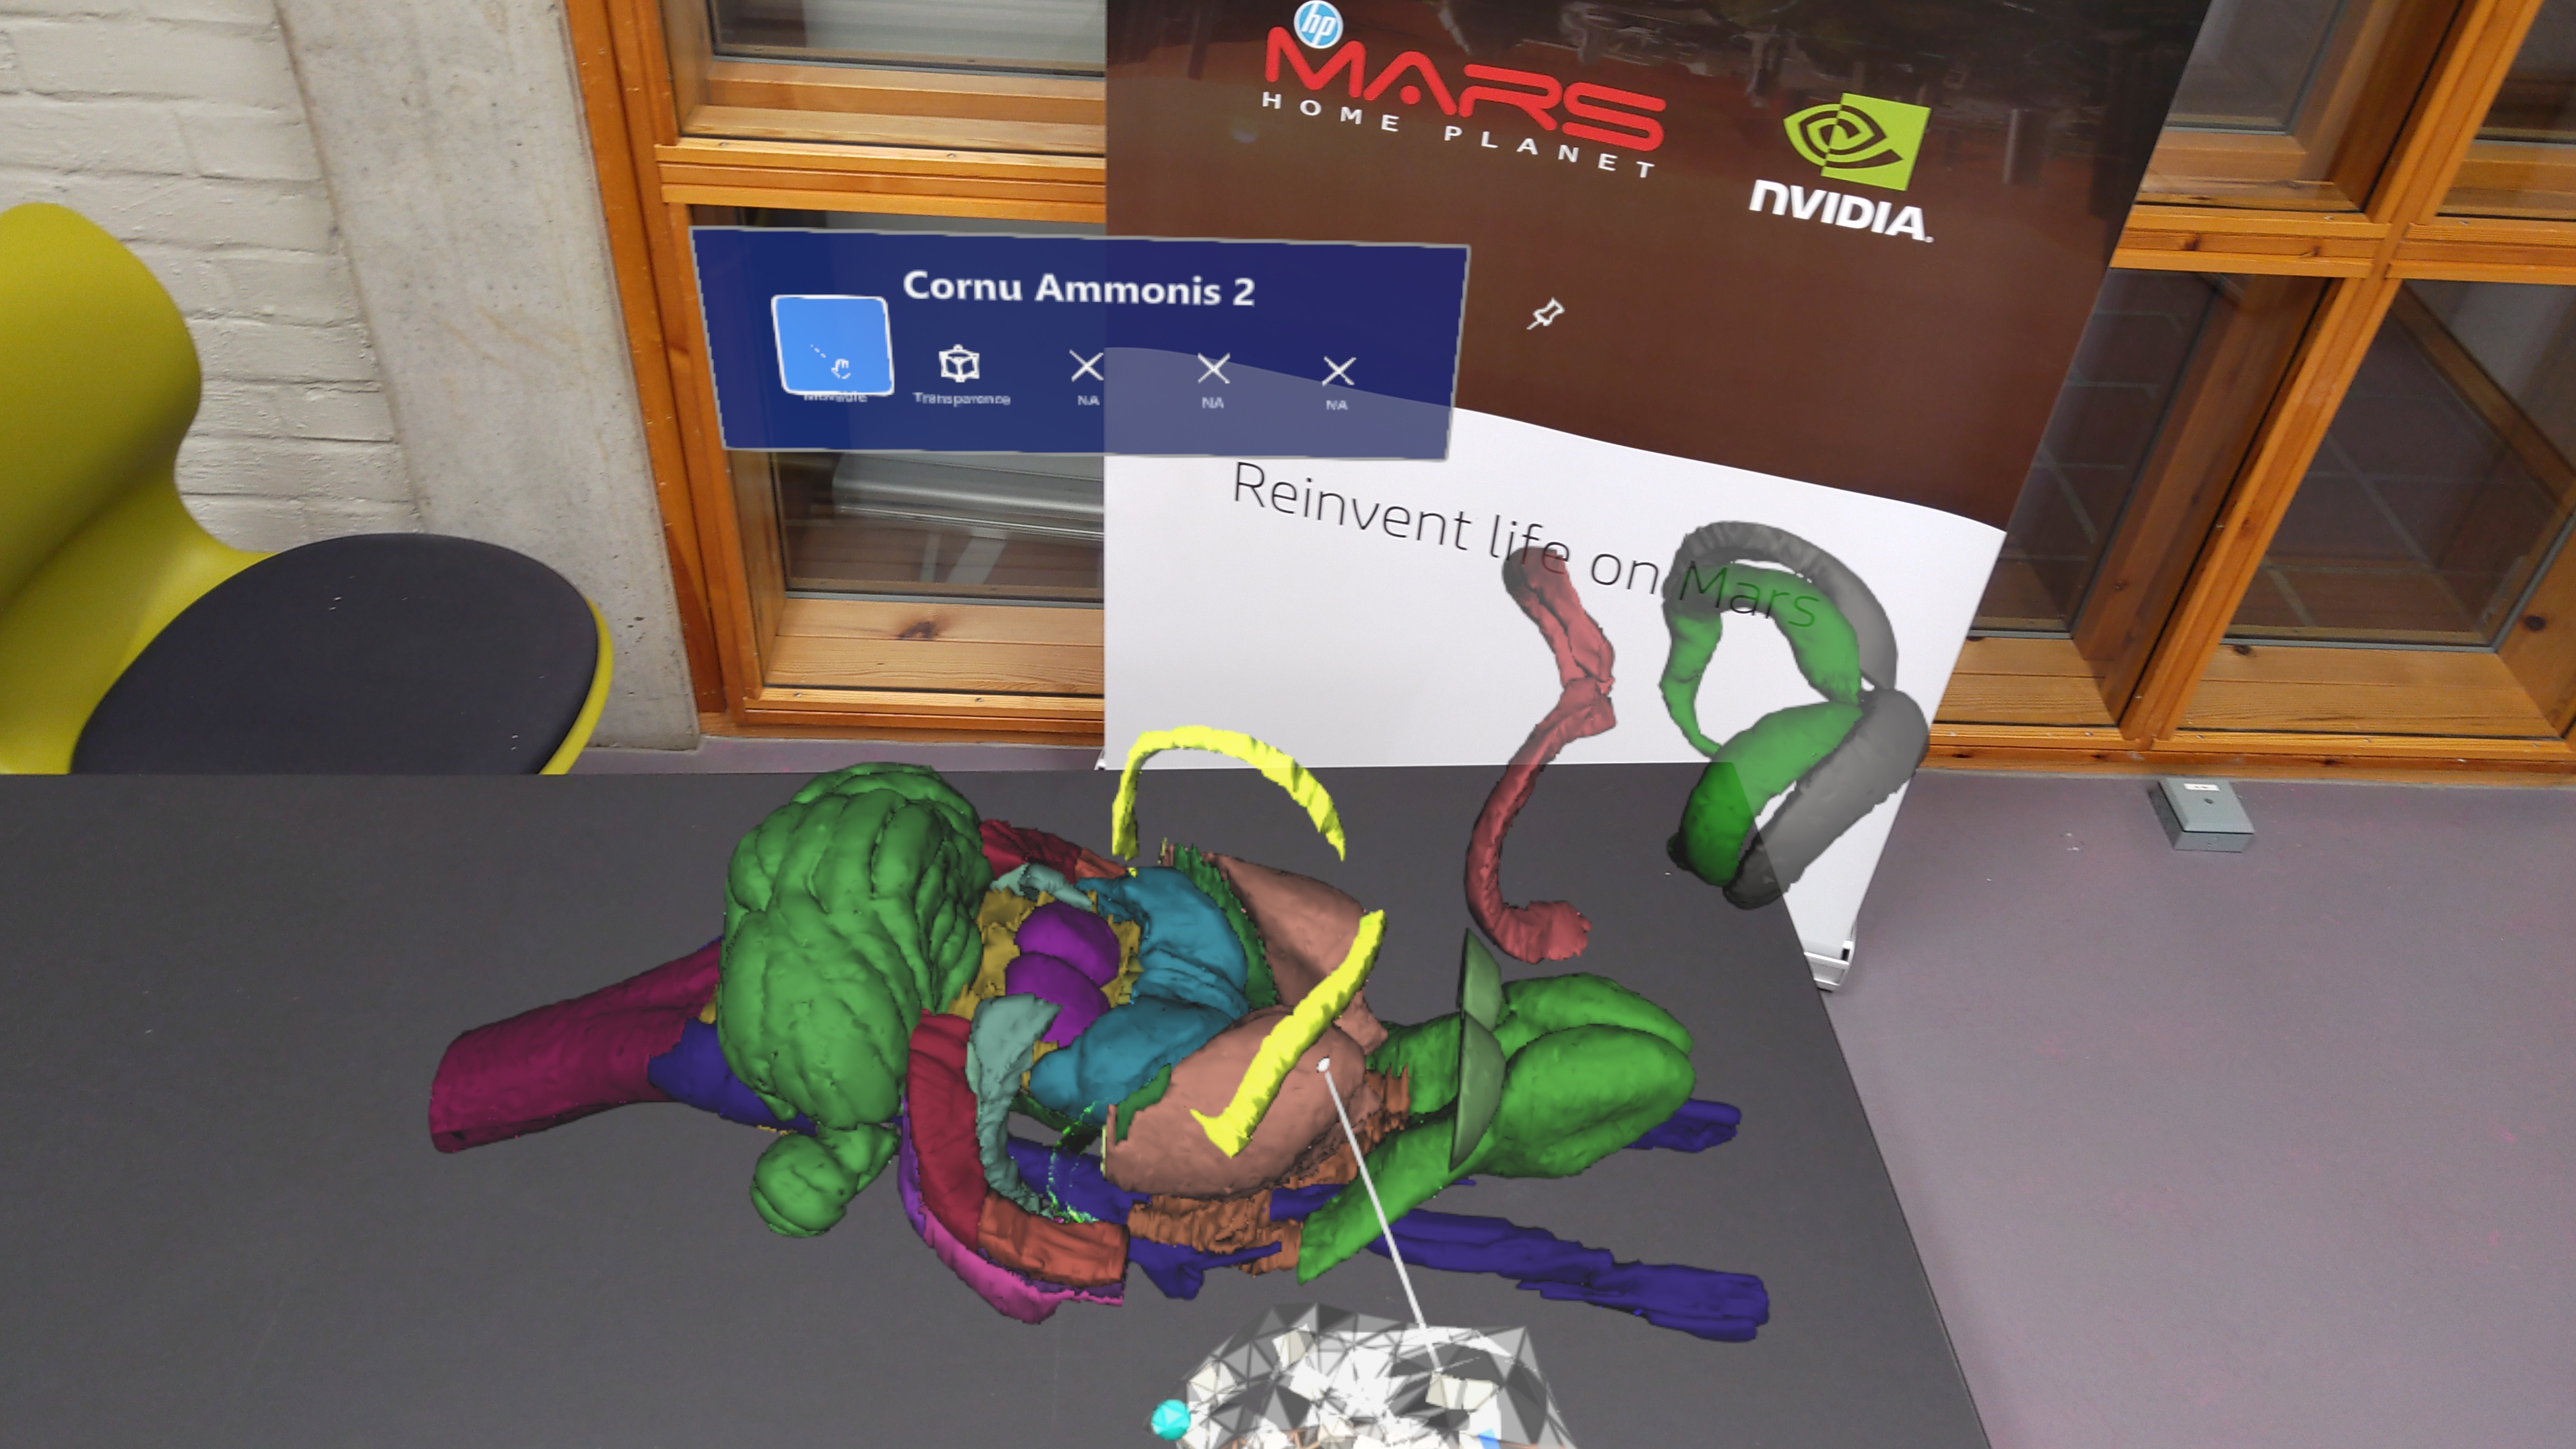
\includegraphics[width=0.5\textwidth]{fig/nevrolens/brainpartsout.jpg}
%     \caption{Nevrolens v0.1.3 on HoloLens 2}
% \end{figure}


% \begin{figure}[h]\label{fig:nevrolens_android}
%     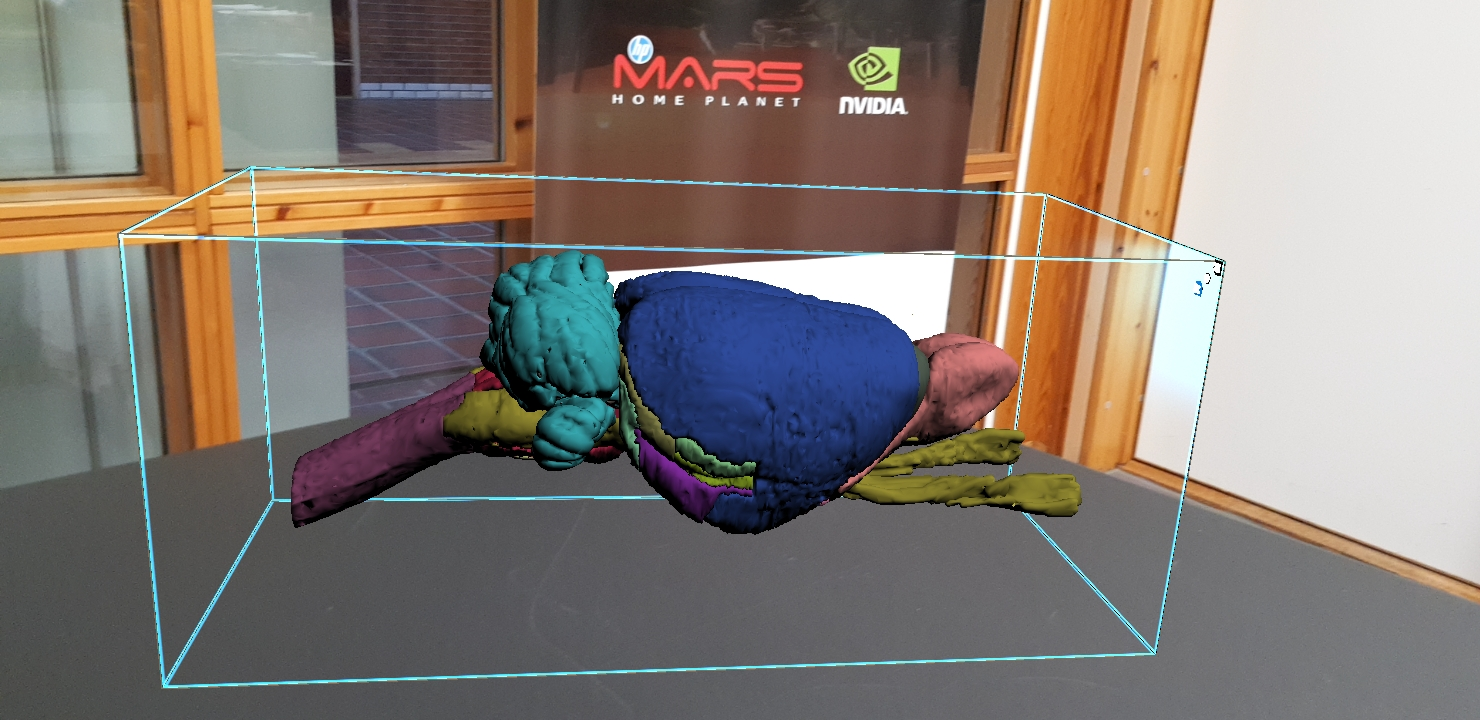
\includegraphics[width=0.5\textwidth]{fig/nevrolens/android_zoom_large.jpg}
%     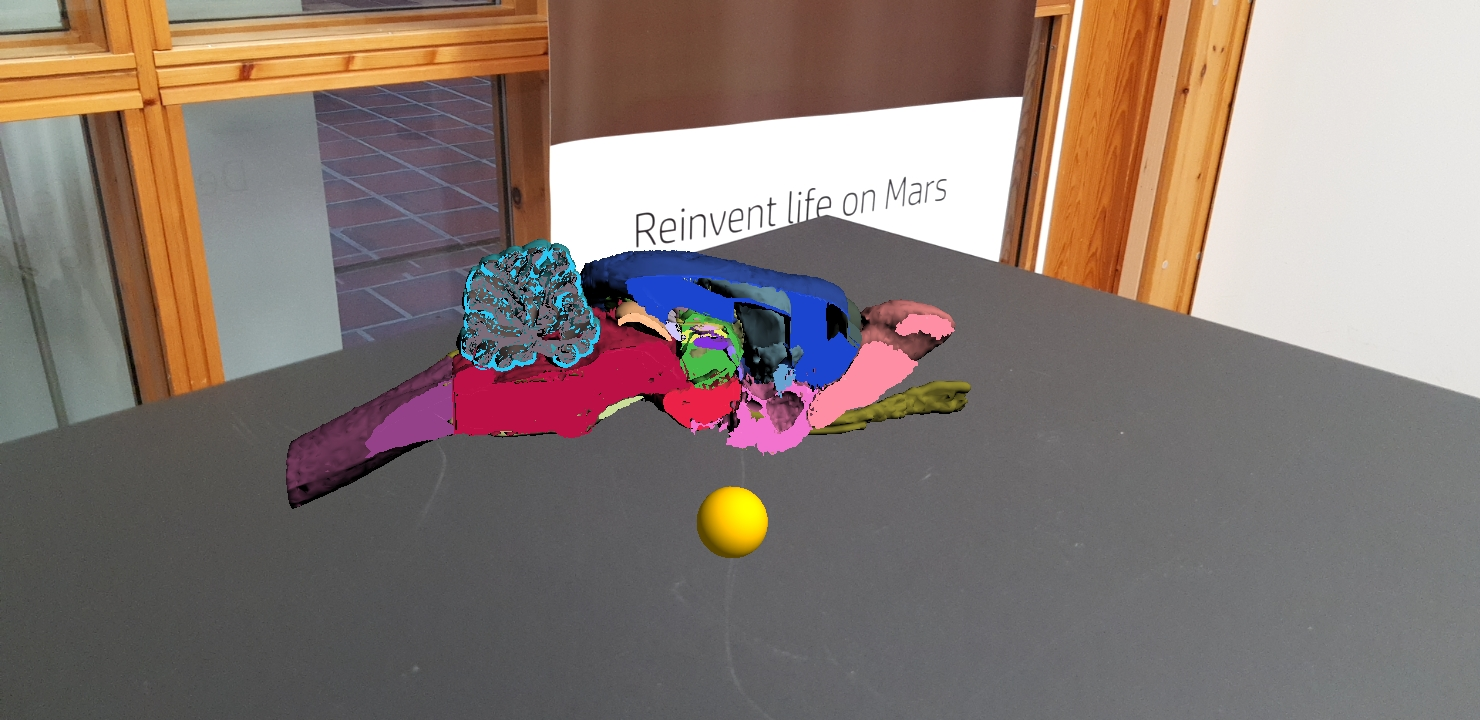
\includegraphics[width=0.5\textwidth]{fig/nevrolens/android_clipping.jpg}
%     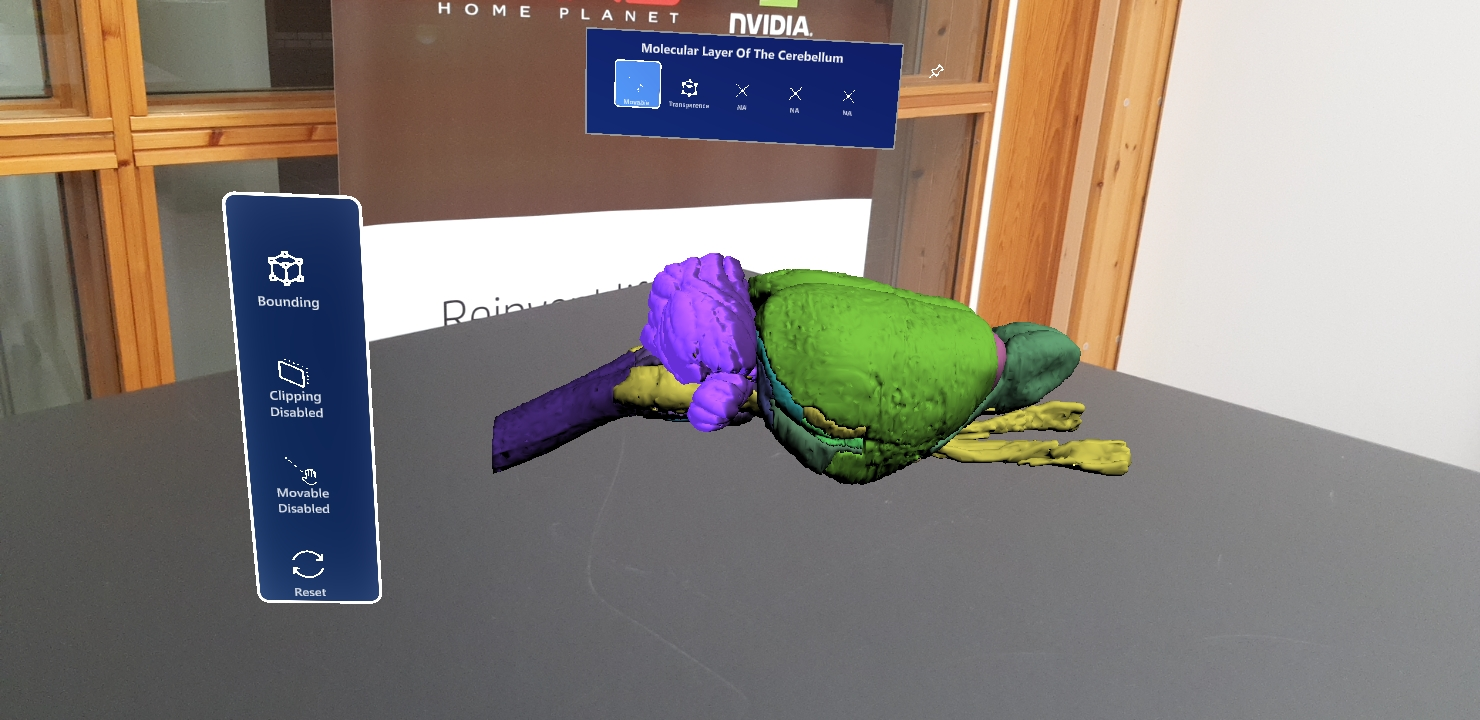
\includegraphics[width=0.5\textwidth]{fig/nevrolens/android_palmmenu.jpg}
%     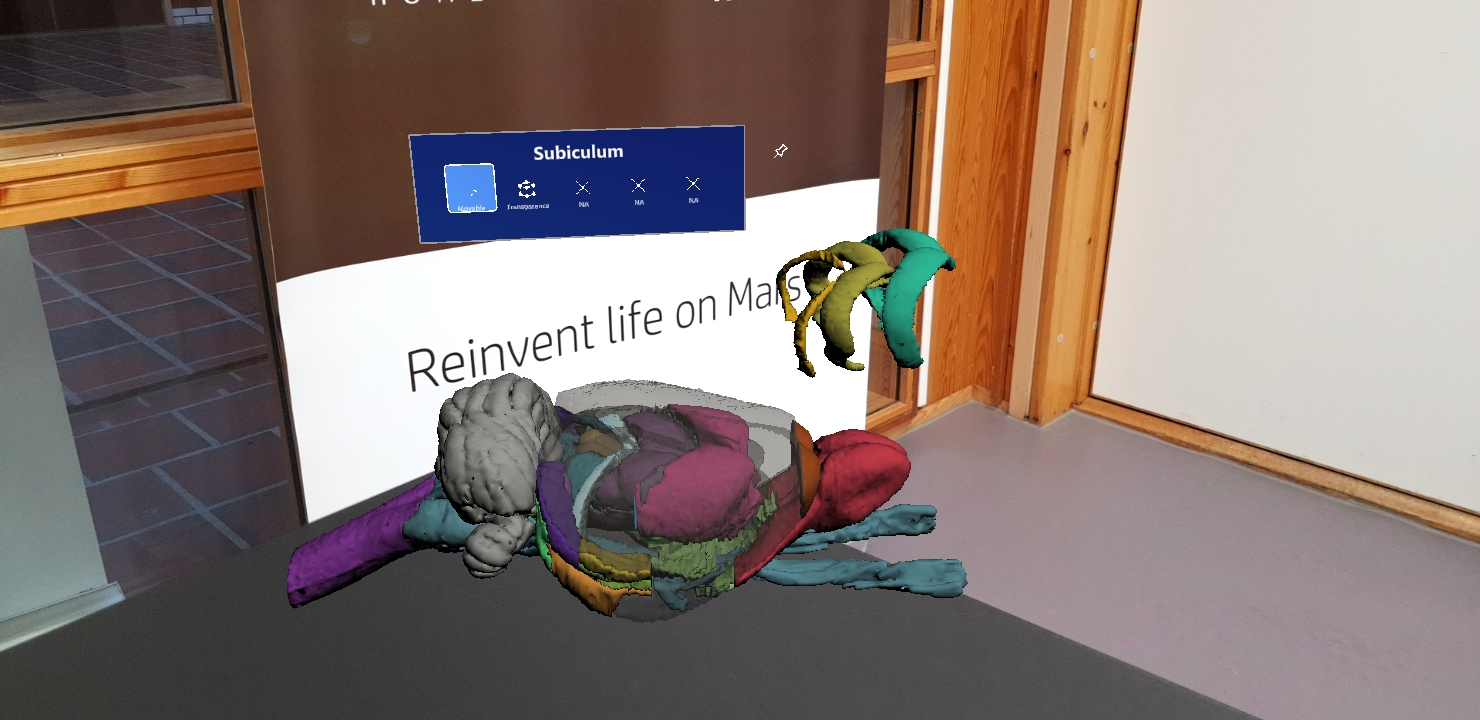
\includegraphics[width=0.5\textwidth]{fig/nevrolens/android_partsout.jpg}
%     \caption{Nevrolens v0.1.3 on Android}
% \end{figure}





% \section{Results}

% Because of the COVID-19 pandemic no user testing has been done this semester, in fact no medical students or professionals have tried the application in-person. Thus, it has been difficult to do formal interviews or gather much feedback, especially regarding interaction. This project is the preliminary work for my master thesis next semester and result gathering will naturally be a much more in focus then. And though no user testing has found place, we have arranged live demoes with \nameref{chap:wdp} over Zoom, which have generated useful feedback. 
% In one such demonstration, I wore a HoloLens 2 and use Nevrolens with guidance from a neuroscientist to extract related regions of the brain and was lectured on their role in behavior. 
% The feedback on its use for a single user, was that there should be a global list menu to toggle different features on each brain part, that there should be ability to increase resolution of a single brain part and some way to visualize microscopical data. 

% % Mostly, the feedback has been positive

% % Success in picking out brain parts, and explaining different structures in the brain. 



% % results from this project are limited.
% !TEX encoding = UTF-8 Unicode
% !TEX root = ../thesis.tex
% !TEX spellcheck = en-US
%%=========================================
\chapter{Conclusion}




%%=========================================
\section{Limitations}

This project rapport is based on work from a 15 credits course, thus there has been time constraints managing the project with other courses and exams. Combined with the busy schedule of the neuroscientists at the Kavli Institute, it has been challenging to gather feedback in the relatively short time frame of this project.
Of course, the COVID-19 pandemic has made physical sharing of the headset problematic, and thus user testing has been difficult. 
In total, there is a very thin basis for results in this project, but this will hopefully be turned around for the master project.


%%=========================================
\section{Discussion}

% The research question the project set out to answer are


This project has mainly focused on implementing the application answering \href{subrq1}{Sub-RQ1}. As such this can be seen as a minimal viable product for exploring Sub-RQ1, and in that capacity it has shown great promise. The basic tools for dissection is implemented and the medical academics at Kavli Institute and UiO sees great potential in its use. 
As for the Sub-RQ2 and 3, there is less work done. However, by building the application for Android, I have shown that the possibility for cross-platform collaboration is open. And it will be worked on for the master thesis, by implementing networking with \nameref{chap:photon}. Sub-RQ3, has not seen any concrete development, I do have some ideas of how it could be implemented with textures generated from a volumetric brain model. 


%%=========================================
\section{Conclusion}

The state of the project now is a small scale proof of concept for a AR application supporting teaching of neuroanatomy and dissection for medical students. There is still no collaboration or microscopic data visualization in the app. However, the biggest problem with the state of the project is the lack of concrete feedback from medical user groups. It has been received very positively by the neuroscientists who has seen the application in use, and they are awaiting more news on the project. The need for exact user testing and user feedback is still large. The project is however progressing nicely, and with further development I believe this project could create impressing results.


%%=========================================
\section{Further Work}\label{chap:futurework}

% \begin{itemize}
%     \item Collaboration, Networking
%     \item Macro+micro implementation
%     \item Importing new models
%     \item Look into volumetric rendering  
% \end{itemize}

There is still a lot of work left on this project, and it will be continues by me. While there is numerous features and fixes which are waiting in the backlog I would like to focus on the overall picture and what has to be in focus to create an collaborative educational experience in AR. 

\begin{itemize}

    \item {
        \textbf{Focus on usability}\\
        Implement better guidance and affordance such that anyone can use the application. To manage this it will be essential to have user testers and testing with medical user groups. This will give feedback on what makes sense and what doesn't.
        
    }
    \item {
        \textbf{Collaboration; implement cross-platform networking}\\
        Networking tools will be required to create a collaborative experience, this will be done using \nameref{chap:photon} to synchronize the HoloLens 2 application with the Android application.
    }

    \item {
        \textbf{Visualize volumetric data}\\
        While the HoloLens 2 does support volumetric rendering, I am pretty sure it is not in an adequate resolution for this project. It will however be explored. Other than that volumetric data could be used as 2D textures mapped on the clipping plane used to cut the brain.
    }

    \item {
        \textbf{Explore ways of using other brains}\\
        \autoref{chap:elden} explains the steps taken by \citet{Elden2017} to use medical imagery in \nameref{chap:vrvis}. An exploration into whether there is a more elegant way of doing this, should be done.
    }

A general focus when continuing this project should be gathering more user data in the form of user tests and interviews, there should be a focus on establishing whether this project can improve learning outcomes for medical students.


\end{itemize}

\section{Future Work}

% Add newer data set WHS rat brain v4

% Add human brain

% Make app more dynamic => Import brain, labels, infoborad text in runtime

% Improve networking stuff => Microsoft Mesh

% Photon Voice

% Improve Android app => menus with android UI should be possible

% More microscopicaldata Sub RQ3

% Desktop or WebGL view app


This section will lay down suggestions for how to further the project. These are based on the authors experience with the research project and on discussions with the neuro specialists and medical students testing the application.

\subsubsection*{Import new data sets}

As described in \autoref{chap:ratbrain} the WHS rat brain is under continuous development and the the near future there will be released a forth version of the brain model, with improved delineation. It is a high priority wish from the Kavli Institute to use this brain model in the application.

To import a WHS brain model as a geometric model is a complicated process, which has been explained by Elden in \autoref{chap:elden}.
The process of exchanging the geometric model used now with a new one however is trivial, but time consuming. A considerable improvement to the application would be the ability to drop in a new model, preferable at run time such that the application wouldn't need to be build and deploy for each model change.
This would enable future WHS versions to easily be added and even other models like human brains could be switched between.  

Another essential feature to reduce the need for new builds is to enable configuration in-app. The application uses three different text files which saves the configuration of clustering, infoboard and labels, all of these should either be possible to upload at run time or configuration with settings UI in-app.

\subsubsection*{Improve networking}
A critical improvement to the application would be to have the initial scene of the application give the user an option of creating a room, joining an existing room or playing offline.
The application as of now will automatically behind the scene, join the existing room or create one if there is none. This gives users less control but more frictionless when testing collaborative features. In a full scale application the user control would probably be preferable.

The networking solution in the application has a considerable amount of bugs and unexpected behavior, this is probably something that is difficult to completely circumvent, but an effort to restructure or fix this should be done.

%todo Microsoft Mesh?

\subsubsection*{Voice chat}

When collaborating in-app remotely the ability to talk to each other would be a great feature, which for a full scale application would be a high priority. 
This can be done with by using Photon Voice for PUN 2.

\subsubsection*{Platform specific input and UI}
There are few limitations in which platforms the application can run on. However, each platform comes with it's own needs for specific input types and UI. The application has been always been developed with HoloLens 2 as the highest priority and that can be seen in most choices taken conserving UI and input handling. Increasing the user experience on Android and even Windows or WebGL (the application is buildable for both, but needs input handling to be usable) should be a priority. Feedback from user testers gave indication that the augmented reality in the android version did not provide an improved user experience and thus disabling camera and spatial features in Android could be seen as an improvement, which could be extended to a desktop application.
A future version of the application running on the web, with WebGL, would probably be possible and further the goal of accessibility.











% Include more chapters as required.
%%=========================================
\appendix
% !TEX encoding = UTF-8 Unicode
%!TEX root = thesis.tex
% !TEX spellcheck = en-US
%%=========================================

\chapter{Acronyms}
\begin{description}
\item[NTNU] Norwegian University of Science and Technology
\item[AR] Augmented Reality
\item[MR] Mixed Reality
\item[XR] Extended Reality
\item[VR] Virtual Reality
\item[HMD] Head-mounted display
\item[WHS] Waxholm Space
\item[GPU] Graphics Processing Unit
\item[SDK] Software Development Kit
\item[COVID-19] Coronavirus Disease 2019
\end{description}
% !TEX encoding = UTF-8 Unicode
%!TEX root = thesis.tex
% !TEX spellcheck = en-US
%%=========================================

\chapter{A geometric model of the rat brain}\label{chap:elden}

This is a section from \citet{Elden2017}, the master thesis about \nameref{chap:vrvis} the VR application this project is loosely inspired by. The section explains how Elden extracted a geometric model of the rat brain from the medical models which is high fidelity volumetric data. I have included it in this report because it gives insight into a specific solution to a problem I face and it explains how a resource I use in this project was created.

\section*{5.2 Exporting segments of a rat brain atlas as geometry
for the Rat Brain model}
The geometric meshes used for the rat brain model were extracted from
a volumetric and segmented atlas. IKT-SNAP was used to export each
segment of the brain as an STL file. These geometric meshes were then
opened in Blender3
to be converted to OBJ or FBX files. 3DS Max imported
the models and performed all modifications made to the geometry and
structure.
ITK-SNAP requires three files to segment and label the models; the
atlas and a segmentation file, both stored as NII files, and a LABEL file
for the labels. When all files are loaded the program lets the user select a
segment to export and generate a geometric hull along the boundary of the
segment. Due to instability experienced with 3DS Max using all 16 GB of
RAM available on the computer used for development, Blender was used
to first convert the files to FBX files. These FBX files caused no issues when
imported into 3DS Max. Since these meshes were too detailed, they needed
to be reduced and transformed in 3DS Max. The meshes were reduced
such that the entire model consisted of 4.5 million triangles. Most of the
meshes had to be transformed such that each segment was where it should
be inside the model. For some reason the exported meshes were of several
relative scales and heights and a lot of manual work went into moving
and scaling the meshes to match the volumetric model seen in ITK-SNAP.
Properly processed, the model was exported as an FBX file and sent to UE4.

% Include more appendices as required.
%%=========================================
\bibliographystyle{apa}
\addcontentsline{toc}{chapter}{\bibname}
\bibliography{refs}  
%%=========================================
%% !TEX encoding = UTF-8 Unicode
%!TEX root = thesis.tex
% !TEX spellcheck = en-US

%This is the Curriculum Vitae
%%=========================================
\addcontentsline{toc}{chapter}{Curriculum Vitae}
\chapter*{Curriculum Vitae}
\hrule
\begin{minipage}[t]{0.65\linewidth}
\begin{tabular}{ll}
Name: & \textbf{Your Name}\\
Gender: & Female\\
Date of birth: & 1. January 1995\\
Address: & Nordre gate 1, N--7005 Trondheim \\
Home address: & King's road 1, 4590 Vladivostok, Senegal\\
Nationality:    & English \\
Email (1): & your.name@stud.ntnu.no\\
Email (2): & yourname@gmail.com\\
Telephone: & +47 12345678\\
\end{tabular} 
\end{minipage}\hfill
\begin{minipage}[t]{0.25\linewidth}

\includegraphics[scale=0.3]{fig/me}\\[1pc] Your picture
\end{minipage}
\hrule

%%=========================================
\section*{Language Skills}
Describe which languages you speak and/or write. Specify your skills in each language.

%%=========================================
\section*{Education}
\begin{itemize}
\item School 1
\item School 2
\item School 3
\end{itemize}

%%=========================================
\section*{Computer Skills}
\begin{itemize}
\item Program 1
\item Program 2
\item Program 3
\end{itemize}

%%=========================================
\section*{Experience}
\begin{itemize}
\item Job 1
\item Job 2
\item Job 3
\end{itemize}

%%=========================================
\section*{Hobbies and Other Activities}         % Your curriculum Vitae     
%%=============================================

\end{document}
